\documentclass[11pt]{article}
\usepackage[T1]{fontenc}
\usepackage{lmodern}
\usepackage[letterpaper,margin=1in]{geometry}
\usepackage{amsmath,amssymb,amsthm,mathtools}
\usepackage{microtype}
\usepackage{booktabs,array}
\usepackage{enumitem}
\usepackage{float}
\floatstyle{ruled}
\newfloat{algorithm}{tbp}{loa}
\floatname{algorithm}{Algorithm}
\newenvironment{algorithmic}[1][1]
{\begin{enumerate}[label=\arabic*:,leftmargin=2em,itemsep=3pt]}
{\end{enumerate}}
\newcommand{\Require}{\item[]\textbf{Input:}\ }
\newcommand{\State}{\item}
\usepackage{tikz}
\usetikzlibrary{arrows.meta,decorations.pathreplacing}
\usepackage[round,authoryear]{natbib}
\usepackage{fancyhdr}
\usepackage{xcolor}
\usepackage[colorlinks=true,linkcolor=blue!40!black,citecolor=blue!40!black,urlcolor=blue!45!black]{hyperref}
\newcommand{\TV}{\operatorname{TV}}
\newcommand{\KL}{D_{\mathrm{KL}}}
\newcommand{\rank}{\operatorname{rank}}
\newcommand{\poly}{\operatorname{poly}}
\newcommand{\negl}{\operatorname{negl}}
\newcommand{\Ber}{\operatorname{Ber}}
\newcommand{\NC}{\mathsf{NC}^{1}}
\newcommand{\TC}{\mathsf{TC}^{0}}
\newcommand{\sig}{\sigma}
\newcommand{\cC}{\mathcal C}
\newtheorem{theorem}{Theorem}
\newtheorem{lemma}[theorem]{Lemma}
\newtheorem{proposition}[theorem]{Proposition}
\newtheorem{corollary}[theorem]{Corollary}
\theoremstyle{definition}
\newtheorem{definition}[theorem]{Definition}
\theoremstyle{remark}
\newtheorem{remark}[theorem]{Remark}
\setlength{\parindent}{1em}
\setlength{\parskip}{3pt}
\setlength{\headheight}{14pt}
\setlist{itemsep=2pt,topsep=4pt}
\pagestyle{fancy}
\fancyhf{}
\fancyhead[L]{\small Learning low-logit-rank distributions}
\fancyhead[R]{\small Mausberg}
\fancyfoot[C]{\thepage}
\hypersetup{pdftitle={Learning Low-Logit-Rank Distributions from Conditional Samples},pdfauthor={Samuel Mausberg}}
\title{\bfseries Learning Low-Logit-Rank Distributions\\from Conditional Samples}
\author{Samuel Mausberg\\[3pt]\normalsize Independent Researcher}
\date{}
\begin{document}
\maketitle
\begin{abstract}
For fully supported binary distributions on length-$T$ strings whose centered next-bit logits have magnitude at most $T$ and rank at most $d$ at every history cut, we prove polynomial-time learning from chosen-prefix next-bit samples at every fixed $d$. The algorithm adds a small amount of fair-bit noise, approximates the resulting analytic logit transformation by a polynomial, and invokes a robust logit learner through a cached sampling simulation. Its costs are $(T+d)^{O(d)}$ at fixed accuracy and confidence, with $\widetilde O_d(T^{6d+15})$ submitted and generated tokens, and it returns a standalone student. A second proof transfers the conditional-sampling theorem for low probability rank through a consistent polynomial surrogate. A specified inverse-polynomial probability floor gives joint polynomial learning as a consequence of the published logit simulation. When the rank grows, strong pseudorandom functions in logarithmic-depth circuits rule out a learner polynomial jointly in $T$ and $d$. The hard teachers carry a linear mismatch counter, which makes every inconsistent-prefix query simulable. We also separate numerical logit simulation from distribution learning: the former requires exponentially many samples even at rank one. Complete token accounting, finite-bit implementations, polynomial sample sufficiency, and a Lean~4 formalization of the main lemmas accompany the proofs.
\end{abstract}

\noindent\textbf{Keywords:} distribution learning, language-model distillation, conditional sampling, logit rank, pseudorandom functions.



\section{Introduction}

Distillation from generated tokens asks a teacher to produce examples and uses those examples to construct a student that can generate on its own. A teacher may also accept a chosen prefix before it produces its next token. This access reveals more than independent training examples, but it does not reveal the numerical probabilities or logits that produced an answer. We study the computational consequences of this distinction for low-logit-rank distributions. Accuracy is measured in total variation (TV), the largest absolute difference between the teacher's and student's probabilities of the same event.

Low logit rank describes linear relations among the teacher's conditional log odds across histories and continuations. It does not posit a small neural-network architecture. Golowich, Liu, and Shetty (GLS) introduced this structural view and proved learning guarantees with numerical logit queries \citep{gls2,gls1}. The binary setting already raises a sharp question. Can a learner recover an accurate generator using only one independently sampled next bit at each chosen prefix?

The answer depends on how rank and conditional probabilities are bounded. If every conditional probability has a specified inverse-polynomial lower bound, the existing approximate-logit simulation is polynomial. Our main positive result goes further: every fixed constant logit rank is learnable in polynomial time even when some conditional probabilities are exponentially small in the sequence length. The main proof combines exactly simulatable token noise with polynomial approximation of the resulting logits. An independent proof constructs a comparison distribution with low probability rank. Both use a rank increase that is polynomial when the original rank is fixed.

When the rank grows, a different conclusion holds under a standard cryptographic assumption. We construct fully supported teachers with polynomially bounded logits and rank at most $n+7$ whose accurate distillation would distinguish a strong pseudorandom function from a random function. A mismatch counter makes every inconsistent-prefix sampling query simulable. The resulting student is tested through one ordinary sample, so the reduction applies to arbitrary standalone generators.

\begin{figure}[t]
\centering
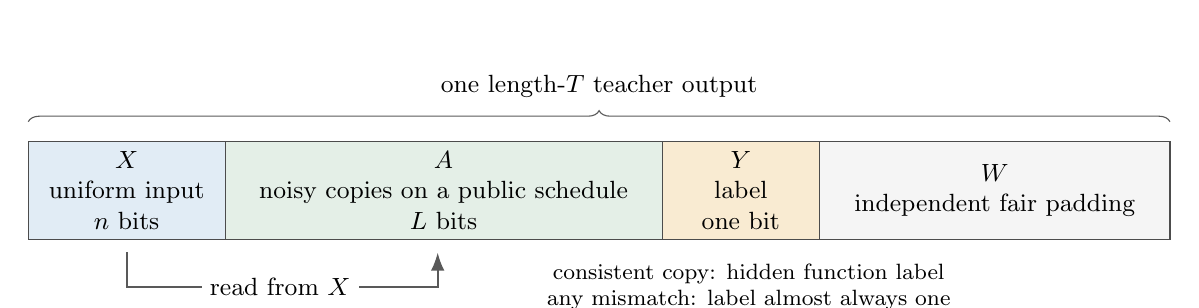
\begin{tikzpicture}[x=1cm,y=1cm,>=Latex,font=\small]
\definecolor{inputfill}{RGB}{225,236,245}
\definecolor{copyfill}{RGB}{228,239,231}
\definecolor{labelfill}{RGB}{249,235,210}
\draw[fill=inputfill,draw=black!70] (0,0) rectangle (2.5,1.25);
\draw[fill=copyfill,draw=black!70] (2.5,0) rectangle (8.05,1.25);
\draw[fill=labelfill,draw=black!70] (8.05,0) rectangle (10.05,1.25);
\draw[fill=black!4,draw=black!70] (10.05,0) rectangle (14.5,1.25);
\node[align=center] at (1.25,.63) {$X$\\uniform input\\$n$ bits};
\node[align=center] at (5.275,.63) {$A$\\noisy copies on a public schedule\\$L$ bits};
\node[align=center] at (9.05,.63) {$Y$\\label\\one bit};
\node[align=center] at (12.275,.63) {$W$\\independent fair padding};
\draw[->,thick,black!65] (1.25,-.16) -- (1.25,-.6) -- (5.2,-.6) -- (5.2,-.16);
\node[fill=white,inner sep=3pt] at (3.2,-.6) {read from $X$};
\draw[decorate,decoration={brace,amplitude=4pt},black!65] (0,1.5) -- (14.5,1.5);
\node[above] at (7.25,1.68) {one length-$T$ teacher output};
\node[anchor=north,align=center,font=\footnotesize] at (9.15,-.18)
{consistent copy: hidden function label\\any mismatch: label almost always one};
\end{tikzpicture}
\caption{The teacher used for the growing-rank conditional lower bound. The input $X$, copy word $A$, label $Y$, and padding $W$ are the four consecutive token blocks. A linear mismatch count controls the label distribution on every submitted prefix, including a prefix that was not generated by the teacher. Section~\ref{sec:hardness} specifies the lengths, probabilities, and hidden computation.}
\label{fig:teacher}
\end{figure}

\subsection{Results and their scope}

Let $\mathcal C_{T,d}$ denote the binary length-$T$ distributions defined precisely in Section~\ref{sec:model}: their scalar centered logits have magnitude at most $T$, and the matrix of future logits has rank at most $d$ at each fixed-length cut. Training is charged for all submitted prefix bits and all returned bits. A student is a finite probabilistic program that generates using its own random bits and never consults the teacher.

\begin{theorem}[Learning at fixed rank]\label{thm:fixed}
There is a uniform randomized learner which, for every $T\ge32$, $d\ge1$, $P\in\mathcal C_{T,d}$, and rational $0<\varepsilon,\delta<1/2$, outputs a standalone sampler $Q$ satisfying
\[
\Pr\{\TV(P,Q)\le\varepsilon\}\ge1-\delta.
\]
Its training bit operations, submitted and returned tokens, output description length, and worst-case generation cost are bounded by
\[
\left(T+d+\log\frac1{\min\{\varepsilon,\delta\}}\right)^{O(d+1)}
\poly\!\left(\frac1{\min\{\varepsilon,\delta\}}\right).
\]
In particular, all these costs are polynomial for every fixed constant $d$.
The numerical-input convention in Section~\ref{sec:model} applies.
\end{theorem}

The main algorithm uses the robust numerical learner of \citet{gls2}. For fixed accuracy and confidence, its total token bound is $\widetilde O_d(T^{6d+15})$, where the subscript allows constants and logarithmic powers depending on fixed $d$. Appendix~\ref{sec:probability-route} gives an independent proof using the probability-rank learner of \citet{liu-moitra}, and Appendix~\ref{sec:alphabet} extends fixed-rank learnability to finite alphabets. The dependence on $d$ is in the exponent; the theorem does not give a polynomial bound jointly in $T$ and $d$.

\begin{theorem}[A specified probability floor; consequence of GLS]\label{thm:floor}
Suppose $T\ge32$, $P\in\mathcal C_{T,d}$, and a supplied rational $\gamma\in(0,1/2]$ satisfies
\[
\gamma\le P(1\mid h)\le1-\gamma
\quad\text{for every }|h|<T.
\]
Then conditional next-bit samples suffice for learning to TV error $\varepsilon$ and failure probability $\delta$, for rational $0<\varepsilon,\delta<1/2$, with all required costs polynomial in $T,d,\gamma^{-1},\varepsilon^{-1},\log(1/\delta)$. With the spanner implementation in Appendix~\ref{sec:finite-bit-gls}, the bounds are
\[
\widetilde O\!\left(\frac{T^{13}d^6}{\gamma\varepsilon^4}\right)
\quad\text{next-bit replies, and}\quad
\widetilde O\!\left(\frac{T^{14}d^6}{\gamma\varepsilon^4}\right)
\quad\text{charged teacher tokens}.
\]
The student has polynomial description length and worst-case generation cost.
The same numerical-input convention applies.
\end{theorem}

Here $\widetilde O$ suppresses powers of logarithms in the displayed parameters. This is an audited consequence of \citet[Theorem~5.11 and Remark~5.8]{gls2}, rather than a new bounded-probability learning principle. The quantitative improvement uses a proved compression bound for the spanner routine and counts the total number of future columns added across cuts. For each fixed $k$ and fixed $c>0$, it applies to the floor $\gamma=cT^{-k}$. A constant floor is included. Allowing the exponent of an unspecified polynomial to vary without a common bound would be a different uniformity requirement.

\begin{theorem}[Conditional obstruction when rank grows]\label{thm:hardness}
If strong Boolean pseudorandom functions with fixed-key logarithmic-depth circuits exist, no uniform learner has costs polynomial jointly in $T,d$ and succeeds with probability $0.99$ at TV error $0.01$ for every $T\ge32$, $1\le d\le T^2$, and $P\in\mathcal C_{T,d}$. Naor--Reingold's finite-field decisional Diffie--Hellman assumption is sufficient for this conclusion.
\end{theorem}

The reduction underlying Theorem~\ref{thm:hardness} is unconditional. A putative learner would produce distinguishing advantage at least $0.4801-o(1)$. The security assumption is stated in Section~\ref{sec:hardness}. It concerns computation, not the amount of sample information: Appendix~\ref{sec:sample-upper} gives polynomial sample sufficiency with an exponential search, and implements that search in $\mathsf{FP}^{\mathsf{NP}}$, deterministic polynomial time with an NP decision oracle.

The two positive regimes are consistent with exponentially large exact probability rank. Section~\ref{sec:separation} gives a rank-two logit example with a constant probability floor and probability rank $2^{\lfloor(T-1)/2\rfloor}$. Section~\ref{sec:scalar} separately proves an $\Omega(e^{2T}/\xi^2)$ lower bound for estimating one centered logit to additive error $\xi$, already at rank one. Those scalar examples are easy to approximate as distributions. Numerical oracle simulation and distribution learning therefore have different costs. With explicit token constants, Appendix~\ref{sec:crossover} proves a tenfold comparison for every $T\ge2048$ at $d=1$ and $\varepsilon=\delta=0.01$. Both procedures receive the same explicit teacher: our deterministic training-token cap is at most one tenth of the complete faithful GLS sampling simulation's expected training replies. The argument uses a root-logit query required by the published procedure.

\newpage
\subsection{The conditional-sampling question}

\citet[Problem~6.2, printed p.~34]{gls2} ask:
\begin{quote}
Can we learn (approximately) low-logit rank models to error $\epsilon$ in $\poly(T,d,|\Sigma|,\alpha,1/\delta,1/\epsilon)$ time using only a conditional sampling oracle?
\end{quote}
In that statement $\Sigma$ is the token alphabet and $\alpha$ bounds the norms in a low-rank factorization. Their Remark~5.8, on printed p.~32, concludes with ``with an overhead of $\poly(e^{\lambda},|\Sigma|,\log(1/\delta),\epsilon^{-1})$.'' More precisely, it gives a per-logit estimate from
\[
O\!\left(e^{2\lambda}|\Sigma|\log(|\Sigma|/\delta)/\epsilon^2\right)
\]
conditional samples when the centered logits have magnitude at most $\lambda$. In the binary case with probability floor $\gamma$, $e^{2\lambda}=(1-\gamma)/\gamma$. Theorem~\ref{thm:floor} follows from this regime of their method. Theorem~\ref{thm:fixed} avoids the exponential logit dependence by a different reduction, while Theorem~\ref{thm:hardness} rules out the fully polynomial conclusion under the stated cryptographic assumption, already for an exact-rank subfamily.

\subsection{Relation to earlier distribution-learning hardness}

\citet{kmrrss} distinguish evaluation of point probabilities from generation of samples. Their noisy-parity result for probabilistic automata, Theorem~16, concerns evaluators. Their Theorem~17 uses pseudorandom-function graph distributions to obtain generator hardness for polynomial-size circuits under a relative-entropy error criterion. Its test of a fresh generated input-output pair is the antecedent of our sampler test. We add a bounded-logit, low-rank sequential encoding and a simulation of all chosen-prefix queries. Total-variation generator hardness from strong pseudorandom functions is treated by \citet{sweke}.

\citet[Section~1.3]{mossel-roch} encode noisy parity in a four-state, time-inhomogeneous hidden Markov model. Their learning task uses independent complete observations and proper model output; the noisy-parity evaluator reduction applies because the output model permits probability evaluation. Neither that access model nor that output requirement is the one studied here. Appendix~\ref{sec:parity} makes the difference explicit: the usual noisy-parity distribution has cutwise logit rank one and is learned by repeated basis-vector prefix queries. A lower bound on observable next-token probabilities also does not imply the nonsingularity assumptions in their positive HMM theorem.

\citet[Section~3]{angluin} explain why a membership-query reduction must answer strings outside the image of its example encoding. Repeated-word encodings are a specific concern there. Our mismatch counter implements that requirement inside a fully supported probabilistic teacher. The generic ideas of graph-distribution testing and invalid-query simulation are established; the low-logit-rank construction and its quantitative adaptive simulation are proved below.

Both positive reductions use polynomial feature expansion, a standard source of matrix-rank bounds; see, for example, \citet[Example~1.2]{budzinskiy}. \citet[Lemma~3.2]{alman-song} use this principle to accelerate attention computation from given query and key matrices. Here the factors are unknown, and the additional issue is transfer from sampled continuations to an accurate standalone generator. Their sequential consistency matters. Each defines one distribution across all cuts, and uniform conditional approximation permits the required adaptive oracle comparison. The main proof uses exact-rank robust logit learning. The alternative invokes the probability-rank theorem of \citet{liu-moitra}, without assuming that the original teacher has low probability rank.


\section{Model and preliminary facts}\label{sec:model}

Write $\{0,1\}^t$ for strings of length $t$, $\{0,1\}^{<t}$ for shorter strings, and $hf$ for concatenation. The empty string is $\varnothing$. A length-$T$ distribution $P$ has \emph{full support} if $P(z)>0$ for every $z\in\{0,1\}^T$. Consequently, every prefix has positive probability and every conditional used below is defined.

For $|h|<T$, let $p_P(h)=P(1\mid h)$ and define the scalar centered logit by
\[
\ell_P(h)=\frac12\log\frac{p_P(h)}{1-p_P(h)}.
\]
All logarithms are natural unless their base is shown. Define $\sigma(u)=(1+e^{-u})^{-1}$, so $p_P(h)=\sigma(2\ell_P(h))$. The full binary centered-logit vector is $(-\ell_P(h),\ell_P(h))$.

At cut $t$, define the real matrix
\[
H_t(P)=\bigl(\ell_P(hf)\bigr)_{
h\in\{0,1\}^t,\ f\in\{0,1\}^{<T-t}}.
\]
The class $\mathcal C_{T,d}$ consists of fully supported $P$ such that $|\ell_P(h)|\le T$ for every prefix and $\rank H_t(P)\le d$ for every $0\le t<T$. The prefix length is fixed within a matrix. Some definitions also mix prefix lengths in one matrix; we identify explicitly when that stronger convention is relevant.

The \emph{probability rank} of $P$ is the largest rank, over $t<T$, of
\[
G_t(P)=\bigl(P(f\mid h)\bigr)_{
h\in\{0,1\}^t,\ f\in\{0,1\}^{T-t}}.
\]
This is a different invariant. Appendix~\ref{sec:probability-route} uses a comparison distribution with low probability rank. This does not impose an additional assumption on $P$.

The learner may submit any prefix $h$ with $|h|<T$ and receive one independent bit from $P(\cdot\mid h)$. The charge is $|h|+1$ tokens, including the submitted prefix and the reply. Successive replies simulate a complete conditional suffix. Starting from a prefix of length $t$, the charge is exactly
\begin{equation}\label{eq:suffix-charge}
\sum_{j=t}^{T-1}(j+1)
=\frac{T(T+1)-t(t+1)}2.
\end{equation}
A student is a finite probabilistic program using ordinary independent fair random bits. Its description and worst-case generation costs are measured in bits and bit operations. It returns a length-$T$ string and has no access to the teacher. Its distribution is denoted by $Q$.

For distributions on a finite set $\Omega$, their total-variation distance is
\[
\TV(P,Q)=\frac12\sum_{z\in\Omega}|P(z)-Q(z)|
=\max_{E\subseteq\Omega}|P(E)-Q(E)|.
\]
We use the coupling bound $\TV(P,Q)\le\Pr\{U\ne V\}$ whenever $(U,V)$ has marginals $(P,Q)$.

For strictly positive $Q$, the relative entropy is
$\KL(P\Vert Q)=\sum_zP(z)\log(P(z)/Q(z))$.
Accuracy, confidence, and probability-floor parameters are finite binary rationals. Each may be rounded down to a dyadic number within a factor of two before the algorithm starts. Our displayed resource bounds apply to these succinct normalized parameters. If the supplied rational encodings have total length $L_{\rm in}$, add $\poly(L_{\rm in})$ bit operations for reading and normalization. This convention prevents arbitrarily long encodings of, for example, numbers near $1/4$ from being hidden in a bound depending only on their numerical values. The fixed accuracy and confidence in the question have constant encoding length.

\begin{lemma}[Uniform conditional comparison]\label{lem:coupling}
Let $P,\widetilde P$ be fully supported binary length-$T$ distributions with
\[
\sup_{|h|<T}|p_P(h)-p_{\widetilde P}(h)|\le\eta.
\]
At any submitted prefix $h$, their complete conditional suffix laws differ by TV at most $(T-|h|)\eta$. An adaptive algorithm making at most $q$ complete conditional suffix queries has transcript TV at most $qT\eta$ under the two oracles. In particular, $\TV(P,\widetilde P)\le T\eta$.
\end{lemma}
\begin{proof}
Couple the next bits maximally while the two generated suffixes agree. Before the first disagreement, the histories coincide, so the conditional probability of a disagreement is at most $\eta$. Summing over the remaining positions proves the suffix bound. Now couple the learner's coins and proceed while its complete transcripts agree. The next queried prefix then agrees, and the conditional discrepancy of its reply is at most $T\eta$. Summing over the first disagreeing query proves the transcript bound. Coins and the output program may be included in the transcript. No bound on the unconditional probability of a submitted prefix is used.
\end{proof}



\section{Learning with a specified probability floor}\label{sec:floor}

A positive lower bound on every conditional probability makes additive logit estimation inexpensive. The relevant cost is inverse-linear in the probability floor. A crude additive estimate of the probability followed by a global derivative bound would instead lose an unnecessary second inverse power.

\begin{lemma}[Bounded factors]\label{lem:bounded-factors}
A real matrix of rank at most $d$, with every entry in $[-\Lambda,\Lambda]$ and $\Lambda\ge1$, has a rank-$d$ factorization whose history and future vectors both have Euclidean norm at most $\sqrt{d\Lambda}$.
\end{lemma}
\begin{proof}
For positive rank $r\le d$, choose $r$ actual rows of maximum Euclidean $r$-dimensional volume among row bases. This volume is the square root of their Gram determinant. An actual row's coefficient in any basis direction has magnitude at most one: replacing that basis row would otherwise increase volume by that factor. Thus the coordinate vectors have norm at most $\sqrt r$, and the basis-value vector at a column has norm at most $\Lambda\sqrt r$. Multiply the first factor by $\sqrt\Lambda$ and the second by its reciprocal. Rank zero is immediate; pad with zeros if $r<d$.
\end{proof}

For the probability floor $\gamma$, set
\[
\lambda_\gamma=\frac12\log\frac{1-\gamma}{\gamma},\qquad
\Lambda=\max\{1,\lambda_\gamma\}.
\]
The lemma gives the bounded-factor parameter required by \citet{gls2}. Take the integer logit bound $L=1+\lceil\log_2(1/\gamma)\rceil$ and supply $\alpha=dL+1$ to the algorithm. Finding the maximum-volume basis is unnecessary.

\begin{lemma}[Finite-bit logit estimation]\label{lem:floor-estimator}
For $0<\gamma\le1/2$, $0<\xi\le1$, and $0<\zeta<1$, a Bernoulli parameter $p\in[\gamma,1-\gamma]$ has its centered logit estimated to additive error $\xi$, with failure at most $\zeta$, from
\[
m=\left\lceil\frac{48}{\gamma\xi^2}
\left\lceil\log_2\frac4\zeta\right\rceil\right\rceil
\]
samples. The estimate can be a dyadic rational, computed in polynomial bit time.
Both ceilings can be computed by integer comparisons and rational arithmetic.
\end{lemma}
We prove Lemma~\ref{lem:floor-estimator} in Appendix~\ref{sec:proof-floor-estimator}, using multiplicative Chernoff bounds and an elementary series for the logarithm.

The robust logit theorem used below accepts independent complete samples and any fixed numerical oracle whose scalar centered answers differ from the target logits by at most $\xi$ at every prefix. Robustness here means that its learning guarantee tolerates these bounded numerical errors. The oracle need not reveal the target's exact real parameters. Appendix~\ref{sec:finite-bit-gls} records constant-factor corrections and the finite-bit implementation of the source algorithm.

\begin{proof}[Proof of Theorem~\ref{thm:floor}]
Use Algorithm~\ref{alg:gls-explicit}, the exact-rank specialization of \citet[Theorem~5.11]{gls2} specified and proved in Appendix~\ref{sec:finite-bit-gls}. Lemma~\ref{lem:explicit-gls-token-envelope} supplies the numerical parameters and reserves constant fractions of the accuracy and failure budgets. Its oracle-trace hypothesis is cutwise: Definitions~4.4 and~5.6 use a separate fixed-history-length matrix at each cut. Thus its use here does not require the stronger mixed-length rank definition from that paper's introduction. The two binary centered-logit columns are negatives of one another, so our scalar convention has the same rank.

Writing $R_\ell$ for logit calls and $R_s$ for complete-sample calls, the improved request bound and the robust tolerance give
\[
R_\ell+R_s=\widetilde O(T^7d^3/\varepsilon^2),
\qquad
\xi=\widetilde\Theta\!\left(\frac{\varepsilon}{T^3d^{3/2}}\right).
\]
Lemma~\ref{lem:bounded-factors} controls the additional factor parameter by a polynomial. For each previously unseen queried prefix, use Lemma~\ref{lem:floor-estimator} with $\zeta=\delta/(2R_\ell)$ and cache the first estimate on the fixed dyadic grid prescribed by Lemma~\ref{lem:explicit-gls-token-envelope}. Full samples come directly from successive teacher calls. The raw reply bound is
\begin{equation}\label{eq:floor-replies}
R_\ell\left\lceil\frac{48}{\gamma\xi^2}
\left\lceil\log_2\frac{8R_\ell}{\delta}\right\rceil\right\rceil+TR_s.
\end{equation}

Appendix~\ref{sec:floor-completion} completes the proof. It couples the cached estimates to an accurate comparison table, losing at most $\delta/2$ in failure probability despite adaptive queries, and converts~\eqref{eq:floor-replies} into the stated token bound.
\end{proof}

Appendix~\ref{sec:parity} explains why a noisy-parity assumption does not give hardness in this access model.


\section{Fixed-rank learning by smoothing the sampled tokens}\label{sec:fixed-rank}

The learner first adds a small amount of independent noise to each sampled next bit. This creates an exactly simulatable comparison oracle whose conditional probabilities are bounded below. Smoothing can increase logit rank. We control that increase by approximating the smoothing transformation with a polynomial and use the robust logit learner on a second comparison distribution. Only its rank bound enters the algorithm.

\subsection{An exactly simulatable smoothed teacher}

For a dyadic $\tau\in(0,1/2)$, define $P^\tau$ by
\[
P^\tau(b\mid h)=(1-\tau)P(b\mid h)+\tau/2.
\]
One conditional bit from $P^\tau$ is sampled exactly as follows. With probability $\tau$, return an independent fair bit; otherwise submit $h$ to the given teacher and return its answer. Each branch produces one token. Its worst-case charge, including any submitted prefix, is $|h|+1$. Fair coins and the dyadic branch decision have bounded bit cost.

The conditional probability floor is $\tau/2$. At every prefix the next-bit TV discrepancy from $P$ is at most $\tau/2$, so
\begin{equation}\label{eq:smoothing-tv}
\TV(P,P^\tau)\le T\tau/2.
\end{equation}
Writing $u=\ell_P(h)$, the centered logit of $P^\tau$ is
\begin{equation}\label{eq:softclip}
\psi_\tau(u)=\frac12\log
\frac{(2-\tau)e^{2u}+\tau}{\tau e^{2u}+2-\tau}.
\end{equation}
Its real magnitude is at most
$M_\tau=\tfrac12\log((2-\tau)/\tau)$.

\begin{lemma}[Polynomial approximation of the smoothed logit]\label{lem:softclip-poly}
For $T\ge1$, $\tau\in(0,1/2)$, and $\zeta\in(0,1)$, there is a real polynomial $r$ of degree at most
\[
\left\lceil3T\log\frac{4T(M_\tau+2)}{\zeta}\right\rceil
\]
such that $\sup_{|u|\le T}|r(u)-\psi_\tau(u)|\le\zeta$.
\end{lemma}
\begin{proof}[Proof sketch]
For complex $u$ with $|\operatorname{Im}u|<1/2$, the number $w=e^{2u}$ has argument in $(-1,1)$, so both $(2-\tau)w+\tau$ and $\tau w+2-\tau$ have positive real part. Hence $\psi_\tau$ is analytic in this strip, and an elementary estimate gives $|\psi_\tau|\le M_\tau+2$ there. Set $\rho=1+1/(2T)$. The Bernstein ellipse with parameter $\rho$, scaled by $T$, lies inside the strip. Cauchy's estimate then makes the Chebyshev coefficients of $z\mapsto\psi_\tau(Tz)$ on $[-1,1]$ decay geometrically with ratio $\rho^{-1}$, and the degree-$k$ truncation error is at most $4T(M_\tau+2)\rho^{-k}$. Since $\log\rho\ge1/(3T)$, the stated degree gives error $\zeta$. Appendix~\ref{sec:proof-softclip} gives the full proof.
\end{proof}

\subsection{The rank increase is polynomial at fixed rank}

Choose one polynomial $r$ from Lemma~\ref{lem:softclip-poly} and define a single fully supported distribution $P^\circ$ by its logits
\[
\ell_{P^\circ}(h)=r(\ell_P(h)).
\]
Equivalently, $P^\circ(1\mid h)=\sigma(2r(\ell_P(h)))$ at every prefix. There is no separate choice of distribution for each cut. Since the derivative of $u\mapsto\sigma(2u)$ has magnitude at most $1/2$,
\begin{equation}\label{eq:smoothed-polynomial-tv}
\sup_h|P^\circ(1\mid h)-P^\tau(1\mid h)|\le\zeta,
\qquad
\TV(P^\circ,P^\tau)\le T\zeta.
\end{equation}

\begin{lemma}[Polynomial transformation of the logit matrices]\label{lem:logit-lift}
If $r$ has degree at most $k$ and $P\in\mathcal C_{T,d}$, every cutwise logit matrix of $P^\circ$ has rank at most
\[
D=\binom{d+k}{d}.
\]
Its entries have magnitude at most $M_\tau+\zeta$.
\end{lemma}
\begin{proof}
Fix a cut $t$ and write $\ell_P(hf)=\langle x_h,a_f\rangle$ with $x_h,a_f\in\mathbb R^d$. The transformed entry $r(\langle x_h,a_f\rangle)$ is a polynomial of total degree at most $k$ in the same coordinates $x_h$, for every future $f$. Expand in the monomials $x^\alpha$ with $\alpha\in\mathbb N^d$ and $\sum_i\alpha_i\le k$. Their number is $\binom{d+k}{d}$: append the slack coordinate $k-\sum_i\alpha_i$ and count compositions into $d+1$ nonnegative parts. This gives a factorization through $D$ features. The magnitude bound follows directly from the uniform approximation.
\end{proof}

\subsection{Algorithm and complete oracle transfer}

We use Algorithm~\ref{alg:gls-explicit}, a fully specified exact-rank version of the robust learner of \citet{gls2}. Lemma~\ref{lem:explicit-gls-token-envelope} supplies numerical constants, finite-bit parameter choices, and a separate proof of termination. For a target of rank at most $D$ and logit magnitude at most an integer $L$, set $\alpha=DL+1$. The bounded-factor hypothesis follows from Lemma~\ref{lem:bounded-factors}.

Write $R_\ell,R_s$ for the numerical-logit and complete-sample request caps, $\xi$ for the robust tolerance, and $W$ for the full sampling simulation's training-token count. With
\begin{equation}\label{eq:gls-polynomial-envelope}
V=\frac{2TDL}{\varepsilon\delta},\qquad C_q=52,
\end{equation}
the explicit implementation satisfies
\[
R_\ell+R_s\le V^{22},\qquad \xi^{-1}\le V^{11},\qquad
W\le V^{C_q}.
\]
The last bound uses the smoothing floor at least $\varepsilon/(32T)$ established below, and includes submitted tokens, returned tokens, and local smoothing coins. Training bit operations, output description length, and worst-case generation bit operations are bounded by $V^{C_{\rm bit}}$ for a separate universal constant $C_{\rm bit}$. Only the numerical constant $C_q$ enters the approximation parameter choice.

Choose
$\tau=2^{-\lceil\log_2(8T/\varepsilon)\rceil}$, so
$\varepsilon/(16T)\le\tau\le\varepsilon/(8T)$, and put
\begin{equation}\label{eq:smooth-parameters}
\begin{gathered}
L=\left\lceil\log_2(4/\tau)\right\rceil+3,\qquad
J=\left\lceil\log_2\frac{2TC_q(d+1)L}{\varepsilon\delta}\right\rceil+10,\\
N=100C_q(d+1)J,\qquad
\zeta=2^{-N},\qquad k=8TN,\qquad D=\binom{d+k}{d}.
\end{gathered}
\end{equation}
These are finite, noncircular choices. The polynomial $r$ and the comparison distribution $P^\circ$ are never computed.

\begin{algorithm}[H]
\caption{Fixed-rank learning from sampled tokens}\label{alg:fixed}
\begin{algorithmic}[1]
\Require $T,d,\varepsilon,\delta$ and the given next-bit sampling oracle
\State Compute $\tau,L,J,N,k,D$ from~\eqref{eq:smooth-parameters}.
\State Run Algorithm~\ref{alg:gls-explicit} with rank $D$, logit bound $L$, and the explicit parameters of Lemma~\ref{lem:explicit-gls-token-envelope}.
\State Generate its requested complete samples from the exactly simulated oracle $P^\tau$.
\State For a new numerical-logit query $h$, estimate $\ell_{P^\tau}(h)$ to error $\xi/2$
       with failure at most $\delta/(4R_\ell)$, and cache the dyadic answer.
\State Return its capped standalone dyadic generator, using a fair-bit fallback on failure.
\end{algorithmic}
\end{algorithm}

\begin{proof}[Proof of Theorem~\ref{thm:fixed}]
The integer $L$ exceeds $M_\tau+2$. The definition of $J$ ensures
$\log(4T(M_\tau+2))\le J\le N$, so $k=8TN$ exceeds the degree in Lemma~\ref{lem:softclip-poly}. The logit rank of $P^\circ$ is at most $D$ and its entries have magnitude at most $L$.

The factor $100$ in $N$ gives all three inequalities
\begin{equation}\label{eq:smooth-budget}
\zeta\le\xi/2,\qquad
R_sT\zeta\le\delta/4,\qquad
T\zeta\le\varepsilon/8,
\end{equation}
as we verify in Appendix~\ref{sec:smooth-parameter-check}.

Define independent conceptual estimation groups from $P^\tau(\cdot\mid h)$ for every prefix $h$, independently of all complete samples and learner coins. The estimator in Lemma~\ref{lem:floor-estimator}, with floor $\tau/2$, produces a cached table $A(h)$ on the fixed dyadic grid prescribed by Lemma~\ref{lem:explicit-gls-token-envelope}. If an entry is accurate for $\ell_{P^\tau}(h)$ within $\xi/2$, it is accurate for $\ell_{P^\circ}(h)$ within $\xi$, by Lemma~\ref{lem:softclip-poly} and~\eqref{eq:smooth-budget}. Replace each inaccurate entry by a canonical $\xi$-accurate approximation to $\ell_{P^\circ}(h)$ on that same grid, obtaining a conceptual table $A_{\rm good}$. This replacement is a proof device.

Consider the ideal run with numerical oracle $A_{\rm good}$ and independent complete samples from $P^\circ$. Conditional on any fixed table, Lemma~\ref{lem:explicit-gls-token-envelope} applies. With probability at least $1-\delta/4$, including the reserved numerical and generation tolerances, its output $Q$ satisfies $\TV(P^\circ,Q)\le\varepsilon/2$.

Couple this run to Algorithm~\ref{alg:fixed}. Before the first disagreement, the queries coincide. On each first numerical query to a new prefix, its untouched estimation group fails with probability at most $\delta/(4R_\ell)$. Cached repetitions add no failure chance. Each complete-sample reply can be coupled with disagreement probability at most $T\zeta$, by~\eqref{eq:smoothed-polynomial-tv}. These bounds hold conditional on the entire common past. Thus the training transcripts disagree with probability at most
\[
\delta/4+R_sT\zeta\le\delta/2.
\]
The actual success probability is at least $1-3\delta/4$. On that event,
\[
\TV(P,Q)
\le\TV(P,P^\tau)+\TV(P^\tau,P^\circ)+\TV(P^\circ,Q)
\le\varepsilon/16+\varepsilon/8+\varepsilon/2<\varepsilon.
\]
There is no numerical-oracle coupling at precision $\zeta$. The sampled numerical estimates need only the robust tolerance $\xi/2$. This is essential: $\zeta$ controls the existential polynomial approximation and the complete-sample comparison.

It remains to count resources. Appendix~\ref{sec:smooth-parameter-check} combines the request bound~\eqref{eq:improved-gls-queries} and the robust tolerance with Lemma~\ref{lem:floor-estimator} at the smoothing floor $\tau/2$ to obtain the token rate~\eqref{eq:smooth-token-rate}. With $D\le\nobreak(801C_q(d+1)TJ)^d$, every cost then obeys the bound of Theorem~\ref{thm:fixed}.
\end{proof}

The original teacher may still have logits of magnitude $T$ and exponentially small conditional probabilities. Smoothing is an operation on sampled tokens, and its TV cost is included in the guarantee for that original teacher. The price for making the oracle numerically accessible is the rank increase to $D$. This increase is polynomial for fixed $d$ and prevents the argument from giving a bound polynomial jointly in $T$ and $d$.
Appendix~\ref{sec:crossover} gives a numerical tenfold cost comparison with faithful numerical logit simulation.


\section{A computational obstruction when rank grows}\label{sec:hardness}

We now prove Theorem~\ref{thm:hardness}. The construction in Figure~\ref{fig:teacher} uses repeated copies to carry a hidden computation. Its distinctive requirement is that the learner may submit inconsistent copies directly. A nonnegative counter ensures that every such label query is nearly independent of the secret.

\subsection{The cryptographic premise and a public read schedule}

A \emph{strong Boolean pseudorandom function} is a family $F_k:\{0,1\}^n\to\{0,1\}$ with efficiently sampled keys, such that uniform probabilistic polynomial-time algorithms with adaptive membership queries have negligible distinguishing advantage between a random $F_k$ and a uniformly random Boolean function. A function of $n$ is negligible if it is smaller than every inverse polynomial for sufficiently large $n$. We assume that each fixed-key function has a bounded-fan-in circuit of depth $O(\log n)$ and polynomial size, with bounds independent of the key. This circuit class is denoted by $\mathsf{NC}^1$.

The finite-field decisional Diffie--Hellman assumption used by \citet{nr} supplies this primitive, as Appendix~\ref{sec:nr-details} explains.

\citet{barrington} converts a depth-$O(\log n)$ circuit into a polynomial-length width-five permutation branching program. Each instruction reads one input coordinate and applies one of two permutations of five states. Its strong form gives identity on one function value and a fixed five-cycle on the other. Hence an initial coordinate vector $v_0$, with one entry equal to one and the others zero, and a sign vector $r\in\{-1,1\}^5$ can read out $2F_k(x)-1$ from the final state. We call such a coordinate vector one-hot. Every sequence of independently chosen instruction bits still produces a one-hot state, even when repetitions are inconsistent.

Let $S(n)$ be a common polynomial instruction bound and pad programs with identities to that length. To eliminate a secret-dependent read schedule, replace an instruction reading $x_i$ by a sweep over all $n$ input coordinates. Use its actual permutation pair at position $i$ and identities at every other position. Prepend one identity sweep. The resulting public schedule has length
\[
L=n(S(n)+1),\qquad i_j=1+((j-1)\bmod n).
\]
Only the permutation pairs $M_{j,0},M_{j,1}$ are hidden. For $a\in\{0,1\}^L$, set
\[
R_k(a)=r^\top M_{L,a_L}\cdots M_{1,a_1}v_0\in\{-1,1\}.
\]
For the consistent word $a(x)=(x_{i_1},\ldots,x_{i_L})$,
\begin{equation}\label{eq:hard-consistency}
R_k(a(x))=2F_k(x)-1.
\end{equation}
The reduction needs only existence of a suitable hidden program for each key. Its simulator never compiles that program or accesses its matrices.

\subsection{Teacher probabilities and exact rank}

Fix $n\ge32$ and define
\begin{equation}\label{eq:hard-parameters}
B=n\log2,\qquad \eta=(1+2^{2n})^{-1},\qquad
T=2n(L+1),\qquad d=n+7.
\end{equation}
Generate $Z=(X,A,Y,W)$ with block lengths $n,L,1,T-n-L-1$. Input and padding bits have logit zero. Copy $j$ has logit $B(2X_{i_j}-1)$. Define the mismatch count
\[
C(X,A)=\sum_{j=1}^L\mathbf1\{A_j\ne X_{i_j}\}.
\]
The label logit is
\begin{equation}\label{eq:hard-mask}
\boxed{\ell_P(XA)=B\bigl(2C(X,A)+R_k(A)\bigr)}.
\end{equation}
These formulas specify the teacher on every prefix. When $C=0$, the label equals $F_k(X)$ with probability $1-\eta$. When $C\ge1$, $2C+R_k(A)\ge1$, so the label is one with probability at least $1-\eta$.

\begin{lemma}\label{lem:hard-teacher}
This teacher belongs to $\mathcal C_{T,n+7}$. It has a polynomial description and rational conditional probabilities with $O(T)$-bit numerators and denominators.
\end{lemma}
\begin{proof}
The logits are finite and satisfy
\[
|\ell_P(h)|\le n\log2\,(2L+1)<2n(L+1)=T.
\]
Full support follows. Each nonzero logit is $Bm$ with integer $|m|\le2L+1$, so its conditional odds are $2^{2nm}$. The integer lengths are $O(nL)=O(T)$.

For rank, use the column state
\[
s(h)=(1,X_1,\ldots,X_n,C,v_1,\ldots,v_5)^\top.
\]
Unfilled input coordinates are zero, $C=0$, and $v=v_0$ initially. Writing an input bit is a linear map because the state contains a constant coordinate. At copy position $j$, after observing $b$, update
\begin{equation}\label{eq:counter}
C\leftarrow C+b+(1-2b)X_{i_j},
\qquad v\leftarrow M_{j,b}v.
\end{equation}
For fixed $b$, this is linear. The counter increment is precisely the mismatch indicator, so earlier mismatches cannot be canceled. The label and padding preserve the state. There are therefore matrices $A_{t,b}$ and vectors $w_t$ with
\[
s(hb)=A_{t,b}s(h),\qquad \ell_P(h)=w_t^\top s(h).
\]
For any cut $t$ and $f=f_1\cdots f_m$ of legal length,
\[
\ell_P(hf)=w_{t+m}^\top A_{t+m-1,f_m}\cdots A_{t,f_1}s(h).
\]
Every column is a functional of the same $n+7$ coordinates. This factors the entire cut matrix, including all future lengths, through dimension $n+7$.
\end{proof}

The rank also grows with $n$: at cut $n$, the columns indexed by the futures $0^{i-1}$, $1\le i\le n$, carry the first $n$ copy logits $B(2X_i-1)$. These are linearly independent functions on $\{0,1\}^n$, so that matrix has rank at least $n$. The construction cannot contradict fixed-constant-rank learnability.

Appendix~\ref{sec:mixed-length} extends the negative theorem to the stronger mixed-history-length convention, with the larger rank bound $T(n+7)\le T^2$.

\subsection{Simulation and the sampler test}

Given membership access to a Boolean function $H$, answer input and padding queries with fair bits, copy queries with the prescribed $X_{i_j}$, consistent-label queries with $H(X)$, and inconsistent-label queries with one. For $H=F_k$, every response law differs from the teacher's law by TV at most $\eta$. First-disagreement coupling therefore bounds the discrepancy of any adaptive $q$-query training transcript by $q\eta$. Prefix parsing is polynomial and each simulated query uses at most one membership query.

\begin{theorem}[Explicit reduction]\label{thm:reduction}
Suppose a uniform learner has polynomial costs jointly in $T,d$ and returns a standalone $Q$ with TV error at most $\varepsilon$, with probability at least $1-\delta$, for every $P\in\mathcal C_{T,d}$. Let $q$ bound its queries at~\eqref{eq:hard-parameters}. There is a uniform polynomial-time membership-query distinguisher with advantage at least
\begin{equation}\label{eq:hard-advantage}
(1-\delta)\left[(1-\eta)^{L+1}
\left(1-\frac q{2^n}\right)-\varepsilon\right]
-q\eta-\frac12.
\end{equation}
\end{theorem}
\begin{proof}
Run the learner with the preceding simulator. Let $\mathcal S$ be the set of inputs used in consistent-label queries during training. Generate one string $(X,A,Y,W)$ from the returned program. Reject malformed output, $A\ne a(X)$, or $X\in\mathcal S$. Otherwise query $H(X)$ and accept exactly when $Y=H(X)$.

Fix a key and a successful real-teacher training transcript. Its structurally defined $\mathcal S$ is now fixed, with size at most $q$. For the event
\[
E_{k,\mathcal S}=\{A=a(X),\ Y=F_k(X),\ X\notin\mathcal S\},
\]
the teacher has mass
\[
P_k(E_{k,\mathcal S})
=(1-\eta)^{L+1}\left(1-\frac{|\mathcal S|}{2^n}\right).
\]
This identity uses a new uniform input and remains true when $\mathcal S$ was selected adaptively. The TV guarantee gives $Q(E_{k,\mathcal S})\ge\max\{0,P_k(E_{k,\mathcal S})-\varepsilon\}$. Average this nonnegative bound over successful transcripts, whose probability is at least $1-\delta$, and then use $|\mathcal S|\le q$. Transferring to simulated training costs at most $q\eta$.

For a uniformly random function $H$, condition on the training transcript, all learner coins, and the generated output. At $X\notin\mathcal S$, the unqueried bit $H(X)$ is still fair and independent. Random-case acceptance is at most $1/2$. Subtracting this bound gives~\eqref{eq:hard-advantage}.

Fixed polynomial caps on training and output generation make the distinguisher total on random-function transcripts outside the learner's promise. It never evaluates a probability under $Q$. The final membership query belongs to the distinguisher, not the student.
\end{proof}

Taking $\varepsilon=\delta=0.01$ yields $0.4801-o(1)$, proving Theorem~\ref{thm:hardness} under the stated assumption. All lengths and query bounds are polynomial in $n$, whereas $\eta\le2^{-2n}$.

The hard teacher is close to an easy generator when the key is known. Let $D_k$ emit uniform $X$, deterministic $A=a(X)$ and $Y=F_k(X)$, and fair padding. Then
\[
\TV(P_k,D_k)=1-(1-\eta)^{L+1}\le(L+1)\eta.
\]
Correct fresh labels therefore occupy almost all ordinary generated mass. Numerical logit queries would reveal the hidden response on an inconsistent word by $R_k(A)=\ell_P(XA)/B-2C(X,A)$; conditional samples conceal it with the proved uniform error. This distinction explains how the distributional lower bound coexists with logit-query learning. Appendix~\ref{sec:weak-error} extends it to every fixed TV error below one.

\begin{corollary}[Smaller power-law logit bounds]\label{cor:power-logits}
Under the same pseudorandom-function assumption, for every fixed $\theta>0$ there is no learner polynomial jointly in $T,d$ for the entire subclass satisfying $|\ell_P(h)|\le T^\theta$. Every next-bit probability in this subclass is at least $(1+e^{2T^\theta})^{-1}$.
\end{corollary}
\begin{proof}
Let $T_0=2n(L+1)$ be the original length and choose a fixed integer $K\ge\max\{1,1/\theta\}$. Append independent fair bits to obtain length $T=T_0^K$. The old cut matrices gain only zero logit columns and later cut matrices vanish. Thus rank remains at most $n+7$, while
$|\ell_P(h)|<T_0=T^{1/K}\le T^\theta$. A learner polynomial in the padded $T,d$ is still polynomial in $n$, because $K$ is fixed. Neither the simulation error nor the fresh-label event changes. The same reduction applies. The conditional probability floor follows from the centered-logit formula.
\end{proof}


\section{Exact probability rank can still be exponential}\label{sec:separation}

Low logit rank does not imply low exact probability rank, even in both positive regimes. The comparison in Appendix~\ref{sec:probability-route} can therefore differ structurally from its target. The following example has logit rank two and a constant probability floor, yet exponential probability rank.

\begin{proposition}\label{prop:cauchy}
For every $T\ge32$ there is $P\in\mathcal C_{T,2}$ with
\[
\frac1{1+e}\le P(b\mid h)\le\frac e{1+e}
\quad\text{for every }h,b,
\]
whose probability rank is at least $2^{\lfloor(T-1)/2\rfloor}$.
\end{proposition}
\begin{proof}
First take $T=2n+1$. For $x\in\{0,1\}^n$, put $s(x)=\sum_{i=1}^n2^{-i}x_i$. Generate independent uniform strings $X,F$ of length $n$, followed by a label with
\[
P(Y=1\mid X=x,F=f)=\sigma(s(x)-s(f)).
\]
The only nonzero logit is $(s(x)-s(f))/2$. Since $0\le s<1$, the probability bounds and full support follow. At any cut, the final logit is a sum of a prefix score and a future score; all columns ending before the label are zero. The full logit matrix is therefore a sum of two outer products and has rank at most two.

At cut $n$, select complete-future columns $(f,1)$. Their matrix is
\[
2^{-n}\operatorname{diag}(a_x)
\left(\frac1{a_x+b_f}\right)_{x,f},
\qquad a_x=e^{s(x)},\quad b_f=e^{s(f)}.
\]
Both lists consist of distinct positive numbers. To prove nonsingularity, suppose a column combination vanishes. The rational function $\sum_f c_f/(z+b_f)$ then vanishes at every $a_x$. After multiplication by $\prod_f(z+b_f)$, its numerator has degree at most $2^n-1$ and has $2^n$ distinct roots. It is identically zero. Evaluating that numerator at $-b_f$ gives $c_f\prod_{g\ne f}(b_g-b_f)=0$, so every $c_f=0$. The selected matrix has rank $2^n$.

For arbitrary $T$, set $n=\lfloor(T-1)/2\rfloor$ and append zero or one independent fair bit. Summing probability columns over this padding recovers the preceding nonsingular matrix. Zero padding logits preserve the logit-rank bound.
\end{proof}

\section{The exponential cost of numerical logit simulation}\label{sec:scalar}

The next proposition concerns an oracle subroutine. It does not contradict fixed-rank distribution learning.

\begin{proposition}[A sharp exponential dependence for scalar estimation]\label{prop:scalar}
Let $T\ge32$ and $0<\xi\le1/6$. Any algorithm that estimates $\ell_P(\varnothing)$ to additive error $\xi$ with probability $0.99$ for every $P\in\mathcal C_{T,1}$ requires more than
\[
\frac{e^{2T}}{30\xi^2}
\]
next-bit oracle replies in the worst case, even with arbitrary adaptive prefix queries.
More specifically, for every such algorithm with a finite deterministic query cap, its expected number of empty-prefix queries exceeds this bound on the particular teacher $P_0$ whose initial logit is $-T$ and whose later bits are independent and fair.
\end{proposition}
\begin{proof}
Compare two teachers whose initial logits are $-T$ and $-T+3\xi$. Every later bit is independently fair under both. Their cutwise logit ranks are at most one, and the logit magnitude bound holds. Write
\[
p_0=(1+e^{2T})^{-1},\qquad p_1=(1+e^{2T-6\xi})^{-1}.
\]
Only an empty-prefix query is informative. Let $A(\theta)=\log(1+e^\theta)$. For $\theta\in[-2T,-2T+6\xi]$, its second derivative is at most $p_1\le e^{6\xi}p_0\le ep_0$. The Bernoulli exponential-family identity and Taylor's theorem give
\[
\KL(\Ber(p_0)\Vert\Ber(p_1))
=A(-2T+6\xi)-A(-2T)-6\xi A'(-2T)
\le18ep_0\xi^2.
\]
Let $N_{\varnothing}$ count the actual empty-prefix queries in a capped adaptive run. Pad after its stopping time with uninformative nonempty-prefix queries, and include its random coins and returned estimate in the transcript. The relative-entropy chain rule gives
\[
\KL(\mathsf{Transcript}_0\Vert\mathsf{Transcript}_1)
=\mathbb E_{P_0}[N_{\varnothing}]\,
  \KL(\Ber(p_0)\Vert\Ber(p_1))
\le18ep_0\xi^2\mathbb E_{P_0}[N_{\varnothing}].
\]
Indeed, conditional on a common past the next submitted prefix is the same function of that past and the shared coins. Its response divergence is the displayed Bernoulli divergence at the empty prefix and zero everywhere else. This identity counts informative bits drawn as parts of complete samples as well as separately requested root bits.

An estimator accurate on both targets gives a test at the midpoint whose acceptance probabilities differ by at least $0.98$. Pinsker's inequality therefore gives transcript divergence at least $2(0.98)^2$. Consequently
\[
\mathbb E_{P_0}[N_{\varnothing}]
\ge\frac{2(0.98)^2}{18e}\frac{1+e^{2T}}{\xi^2}
>\frac{e^{2T}}{30\xi^2}.\qedhere
\]
\end{proof}

The worst-case total reply count is at least this expectation. An algorithm without a finite query cap already has infinite worst-case cost. For failure probability $\delta<1/2$, the capped version of the same proof gives
\[
\mathbb E_{P_0}[N_{\varnothing}]
\ge\frac{(1-2\delta)^2}{9e}\frac{1+e^{2T}}{\xi^2}.
\]
Both teachers in the proof are within $e^{-2T+1}$ of the same generator: emit a zero and then fair bits. Thus faithful numerical simulation needs exponentially many observations even though their distributions admit an immediate constant-accuracy approximation. Together with the upper estimate in Remark~5.8 of \citet{gls2}, the proposition identifies the exponential dependence of that uniform subroutine. It supplies no exponential lower bound for distribution learning.


\section{Consequences and remaining questions}\label{sec:discussion}

The probability floor and the rank answer different computational questions. A supplied inverse-polynomial floor makes numerical logit estimation polynomial, and the existing robust learner then handles growing rank. Without that floor, fixing the rank still suffices: the algorithm permits rank to grow during its internal approximation, at a cost whose exponent depends on the original rank. The hard family has rank between $n$ and $n+7$, so its cryptographic obstruction concerns a growing-rank regime.

For generated-token distillation, rare conditional events matter through their effect on the resulting distribution and through the learner's choice of queries. Proposition~\ref{prop:scalar} requires exponential cost to estimate a rare logit faithfully. The teachers in that proposition are all close to one simple generator. Conversely, the cryptographic construction places the distinguishing labels on almost all generated mass; its obstacle is not an inaccurate estimate of an event that can be discarded within the TV budget.

Appendix~\ref{sec:sample-upper} constructs a finite-bit cover with polynomial logarithmic cardinality and a polynomial-sample likelihood learner, with an exponential search. That search lies in $\mathsf{FP}^{\mathsf{NP}}$ once the random sample has been obtained. Thus a proof of unconditional nonexistence of a joint-polynomial learner would imply $\mathsf P\ne\mathsf{NP}$.

Several quantitative questions remain. The fixed-rank algorithm is an existence result with large polynomial exponents. Its rank increase and the robust learner's costs may admit substantial improvements. For growing rank, the present results do not settle logit magnitudes between $O(\log T)$ and $T^\theta$ for every fixed $\theta>0$. They also do not settle whether the fixed-rank bound can be improved from $T^{O(d)}$ to $f(d)\poly(T)$ for some function $f$. The cryptographic reduction excludes a polynomial choice of $f$ under its assumption, but does not exclude all such parameter dependence.
In particular, the reduction does not prove that distribution learning needs $e^{\Omega(T)}$ queries or time.

All guarantees above concern exact cutwise logit rank unless an approximation is explicitly constructed in a proof. Robustness to an externally supplied average-rank error requires a separate quantitative analysis. No benchmark on trained neural networks or hardware is claimed. Appendix~\ref{sec:audit} describes the finite structural calculations and the Lean~4 formalization, and lists the parts of the argument that remain outside it.


\makeatletter\def\UrlBigBreaks{\do@url@hyp}\g@addto@macro\UrlNoBreaks{\do\:}\makeatother
\begin{thebibliography}{99}

\bibitem[Allamigeon et~al.(2025)Allamigeon, Dadush, Loho, Natura, and V{\'e}gh]{rational-svd}
Xavier Allamigeon, Daniel Dadush, Georg Loho, Bento Natura, and L{\'a}szl{\'o} A.~V{\'e}gh.
\newblock Interior point methods are not worse than Simplex.
\newblock arXiv:2206.08810v4, 2025. Definition~6.13 and Theorem~6.16.
\newblock \url{https://arxiv.org/abs/2206.08810v4}.

\bibitem[Alman and Song(2023)]{alman-song}
Josh Alman and Zhao Song.
\newblock Fast attention requires bounded entries.
\newblock In \emph{Advances in Neural Information Processing Systems}, volume~36, 2023.
\newblock \url{https://arxiv.org/abs/2302.13214}.

\bibitem[Angluin and Kharitonov(1991)]{angluin}
Dana Angluin and Michael Kharitonov.
\newblock When won't membership queries help?
\newblock In \emph{Proceedings of the Twenty-Third Annual ACM Symposium on Theory of Computing}, 1991. Extended abstract, Section~3.
\newblock \url{https://www.cis.upenn.edu/~mkearns/teaching/Crypto/angluin.pdf}.

\bibitem[Balle and Mohri(2015)]{balle-mohri}
Borja Balle and Mehryar Mohri.
\newblock On the Rademacher complexity of weighted automata.
\newblock In \emph{Algorithmic Learning Theory}, 2015.
\newblock \url{https://cs.nyu.edu/~mohri/pub/wfarad.pdf}.

\bibitem[Barrington(1989)]{barrington}
David A.~Barrington.
\newblock Bounded-width polynomial-size branching programs recognize exactly those languages in $\mathsf{NC}^1$.
\newblock \emph{Journal of Computer and System Sciences}, 38(1):150--164, 1989.
\newblock \url{https://doi.org/10.1016/0022-0000(89)90037-8}.

\bibitem[Budzinskiy(2025)]{budzinskiy}
Stanislav Budzinskiy.
\newblock When big data actually are low-rank, or entrywise approximation of certain function-generated matrices.
\newblock \emph{SIAM Journal on Mathematics of Data Science}, 7(3):1098--1122, 2025.
\newblock \url{https://doi.org/10.1137/24M1687133}.
\newblock Author version: \url{https://arxiv.org/abs/2407.03250v4}.

\bibitem[Floyd and Warmuth(1995)]{floyd-warmuth}
Sally Floyd and Manfred Warmuth.
\newblock Sample compression, learnability, and the Vapnik--Chervonenkis dimension.
\newblock \emph{Machine Learning}, 21(3):269--304, 1995.
\newblock \url{https://doi.org/10.1007/BF00993593}.

\bibitem[Golowich et~al.(2025)Golowich, Liu, and Shetty]{gls2}
Noah Golowich, Allen Liu, and Abhishek Shetty.
\newblock Provably learning from modern language models via low logit rank.
\newblock arXiv:2512.09892v1, 2025.
\newblock \url{https://arxiv.org/abs/2512.09892v1}.

\bibitem[Golowich et~al.(2026)Golowich, Liu, and Shetty]{gls1}
Noah Golowich, Allen Liu, and Abhishek Shetty.
\newblock Sequences of logits reveal the low rank structure of language models.
\newblock In \emph{International Conference on Learning Representations}, 2026.
\newblock \url{https://arxiv.org/abs/2510.24966}.

\bibitem[Gr{\"o}tschel et~al.(1981)Gr{\"o}tschel, Lov{\'a}sz, and Schrijver]{ellipsoid}
Martin Gr{\"o}tschel, L{\'a}szl{\'o} Lov{\'a}sz, and Alexander Schrijver.
\newblock The ellipsoid method and its consequences in combinatorial optimization.
\newblock \emph{Combinatorica}, 1(2):169--197, 1981.
\newblock \url{https://ir.cwi.nl/pub/10046/10046D.pdf}.

\bibitem[Kearns et~al.(1994)Kearns, Mansour, Ron, Rubinfeld, Schapire, and Sellie]{kmrrss}
Michael Kearns, Yishay Mansour, Dana Ron, Ronitt Rubinfeld, Robert E.~Schapire, and Linda Sellie.
\newblock On the learnability of discrete distributions.
\newblock In \emph{Proceedings of the Twenty-Sixth Annual ACM Symposium on Theory of Computing}, 1994.
\newblock \url{https://people.csail.mit.edu/ronitt/papers/learndist.pdf}.

\bibitem[Liu and Moitra(2025)]{liu-moitra}
Allen Liu and Ankur Moitra.
\newblock Model stealing for any low-rank language model.
\newblock In \emph{Proceedings of the Fifty-Seventh Annual ACM Symposium on Theory of Computing}, 2025.
\newblock \url{https://doi.org/10.1145/3717823.3718220}.
\newblock Theorem and algorithm numbering here refers to
\url{https://arxiv.org/abs/2411.07536v1}.

\bibitem[Mossel and Roch(2006)]{mossel-roch}
Elchanan Mossel and S{\'e}bastien Roch.
\newblock Learning nonsingular phylogenies and hidden Markov models.
\newblock \emph{Annals of Applied Probability}, 16(2):583--614, 2006.
\newblock \url{https://doi.org/10.1214/105051606000000024}.

\bibitem[Naor and Reingold(2004)]{nr}
Moni Naor and Omer Reingold.
\newblock Number-theoretic constructions of efficient pseudo-random functions.
\newblock \emph{Journal of the ACM}, 51(2):231--262, 2004.
\newblock \url{https://doi.org/10.1145/972639.972643}.

\bibitem[Sweke et~al.(2021)Sweke, Seifert, Hangleiter, and Eisert]{sweke}
Ryan Sweke, Jean-Pierre Seifert, Dominik Hangleiter, and Jens Eisert.
\newblock On the quantum versus classical learnability of discrete distributions.
\newblock \emph{Quantum}, 5:417, 2021.
\newblock \url{https://doi.org/10.22331/q-2021-03-23-417}.

\end{thebibliography}



\clearpage
\appendix


\section{\texorpdfstring{Deferred proofs and details for Sections~\ref*{sec:floor}--\ref*{sec:hardness}}{Deferred proofs and details for Sections 3-5}}\label{sec:deferred}

This appendix contains the proofs and computations deferred from Sections~\ref{sec:floor}--\ref{sec:hardness}, in the order in which the main text uses them. It also contains the noisy-parity calculation referred to in the introduction and in Section~\ref{sec:floor}.

\subsection{Finite-bit logit estimation}\label{sec:proof-floor-estimator}

\begin{proof}[Proof of Lemma~\ref{lem:floor-estimator}]
Let $U$ be the empirical fraction of ones and put $\tau=\xi/4$. Multiplicative Chernoff bounds for both outcomes give
\[
\Pr\{|U-p|>\tau p\text{ or }|(1-U)-(1-p)|>\tau(1-p)\}
\le4e^{-m\gamma\tau^2/3}\le\zeta.
\]
On the complementary event, $\tau\le1/4$ and both logarithmic ratio errors are at most $\tau/(1-\tau)\le\xi/3$. Hence the centered logit of $U$ differs from the true one by at most $\xi/3$.

For a total finite-bit routine, first clip $U$ to $[\gamma/2,1-\gamma/2]$, which has no effect on the good event. Approximate its centered logarithm and dyadically round with total error at most $\xi/2$. One elementary logarithm routine writes a positive rational as $2^jy$ with $1\le y<2$ and uses
\[
\log y=2\sum_{r\ge0}\frac{z^{2r+1}}{2r+1},
\qquad z=\frac{y-1}{y+1}\in[0,1/3).
\]
The same series at $z=1/3$ computes $\log2$. Its geometric tail requires only polynomially many precision bits. The total estimation error is at most $5\xi/6$.
\end{proof}

\subsection{Adaptive caching and token count under a probability floor}\label{sec:floor-completion}

\begin{proof}[Completion of the proof of Theorem~\ref{thm:floor}]
We continue the proof in Section~\ref{sec:floor} from the raw reply bound~\eqref{eq:floor-replies}.
We justify adaptivity without conditioning incorrectly on the estimation event. Conceptually assign independent estimation samples to every possible prefix, independently of the learner's complete samples and coins. Let $A(h)$ be the resulting cached estimate. Define a comparison table $A_{\rm good}$ by replacing every inaccurate entry with a canonical accurate approximation on that same dyadic grid. These replacements are only proof objects. Conditional on any comparison table, the robust logit theorem applies, because the learner's complete samples and coins remain independent of it. Couple the actual and comparison runs. Before their first disagreement, a new prefix has an untouched independent sample group, whose failure probability is at most $\delta/(2R_\ell)$. Repeated prefixes use their cached answer. A union bound bounds the chance of any disagreement by $\delta/2$.

Each logit-estimation reply costs at most $T$ tokens including its prefix. Each complete sample costs $T(T+1)/2$. Multiplying~\eqref{eq:floor-replies} accordingly gives the claimed token bound. The published learner's linear programs and spanner calculations have polynomially many bounded-bit rational coefficients under these dyadic oracle answers. Appendix~\ref{sec:finite-bit-gls} gives the finite-bit implementation and the dyadic, total standalone generator. Reserving the remaining constant fraction of the TV budget for generation rounding completes the proof.
\end{proof}

\subsection{Why a noisy-parity assumption does not give hardness here}\label{sec:parity}

Let $s\in\{0,1\}^n$ be a hidden vector and $\nu\in(0,1/2)$ a fixed noise rate. Generate independent uniform bits $X\in\{0,1\}^n$ and then
\[
Y=\langle s,X\rangle_{\mathbb F_2}\oplus E,
\qquad E\sim\Ber(\nu).
\]
Here $\mathbb F_2$ denotes arithmetic modulo two, and $\oplus$ is addition modulo two. This is the usual noisy-parity distribution. Its observable next-token probabilities lie in $[\nu,1-\nu]$.

In fact its cutwise logit rank is at most one. Every logit before the final label is zero. If $B=\tfrac12\log((1-\nu)/\nu)$, the label logit is $-B(-1)^{\langle s,x\rangle}$. At any input cut, the parity sign factors into a prefix sign and a future sign. The remaining, shorter-future columns are zero, so the entire matrix is an outer product.
It belongs to $\mathcal C_{T,1}$ for $T=n+1\ge\max\{32,B\}$.

For each $i$, query the length-$n$ standard basis vector $e_i$ repeatedly. Each answer equals $s_i$ with probability $1-\nu$. Majority after
\[
r=\left\lceil\frac{2}{(1-2\nu)^2}\left\lceil\log_2\frac n\delta\right\rceil\right\rceil
\]
repetitions has error at most $\delta/n$, by Hoeffding's inequality. Thus $nr$ replies and $n(n+1)r$ charged tokens recover the whole key with failure at most $\delta$. For known dyadic $\nu$, a standalone generator is then exact. For other known noise rates, dyadic approximation gives any requested TV accuracy. If the rate is unknown, repeated queries to $0^n$ estimate it as an ordinary Bernoulli parameter.

This calculation addresses the access distinction in the noisy-parity HMM literature directly. Independent examples cannot be replaced by chosen inputs at no cost, and an arbitrary output sampler does not by itself evaluate an unknown parity on demand.

\subsection{Polynomial approximation of the smoothed logit}\label{sec:proof-softclip}

\begin{proof}[Proof of Lemma~\ref{lem:softclip-poly}]
For complex $u$ with $|\operatorname{Im}u|<1/2$, the number $w=e^{2u}$ has argument in $(-1,1)$. Both $(2-\tau)w+\tau$ and $\tau w+2-\tau$ have positive real part. Their principal logarithms, and hence their difference in~\eqref{eq:softclip}, are analytic in this strip.

Put $c=2-\tau$, $b=\tau$, and $s=|w|$. Triangle bounds and the positive real parts give
\[
\cos(1)\frac bc
\le\frac{|cw+b|}{|bw+c|}
\le\frac1{\cos(1)}\frac cb.
\]
For example, the upper bound follows from
$|cw+b|\le cs+b$, $|bw+c|\ge\cos(1)(bs+c)$, and
$(cs+b)/(bs+c)\le c/b$. The lower bound follows by interchanging numerator and denominator. The two arguments have the same sign and both lie between zero and $\arg w$. Therefore
\[
|\operatorname{Re}\psi_\tau(u)|
\le M_\tau+\tfrac12\log\sec(1),
\qquad
|\operatorname{Im}\psi_\tau(u)|<\tfrac12.
\]
In particular, $|\psi_\tau(u)|\le M_\tau+2$ throughout the strip.

Set $\rho=1+1/(2T)$. The Bernstein ellipse, obtained from $|w|=\rho$ by $z=(w+w^{-1})/2$ and taking its interior, satisfies
$|\operatorname{Im}(Tz)|<1/2$. Thus $F(z)=\psi_\tau(Tz)$ is analytic there and has modulus at most $M_\tau+2$. The Laurent expansion of $F((w+w^{-1})/2)$ has coefficients $c_j=c_{-j}$ with
$|c_j|\le(M_\tau+2)\rho^{-j}$, by Cauchy's coefficient estimate. On $[-1,1]$ this is the Chebyshev series
$c_0+2\sum_{j\ge1}c_jT_j(x)$, where $T_j(\cos\theta)=\cos(j\theta)$. Its degree-$k$ tail is at most
\[
2(M_\tau+2)\sum_{j>k}\rho^{-j}
=4T(M_\tau+2)\rho^{-k}.
\]
The coefficients are real, and $\log\rho\ge1/(3T)$. The stated degree therefore gives error $\zeta$ after rescaling.
\end{proof}

\subsection{Parameter checks and token count at fixed rank}\label{sec:smooth-parameter-check}

\begin{proof}[Completion of the proof of Theorem~\ref{thm:fixed}]
We verify that the factor $100$ in $N$ gives~\eqref{eq:smooth-budget} for the parameters~\eqref{eq:smooth-parameters}, and then count the training tokens.
For the error budget, first observe
\[
D\le(d+800C_q(d+1)TJ)^d
\le\bigl(801C_q(d+1)TJ\bigr)^d.
\]
Also
\[
\log_2C_q+\log_2(d+1)+\log_2T+\log_2L+
\log_2(1/\varepsilon)+\log_2(1/\delta)\le J-11.
\]
Consequently $\log_2D\le3dJ$ and $\log_2V\le(3d+1)J$. For the first inequality in~\eqref{eq:smooth-budget}, use $\xi^{-1}\le V^{C_q}$ and
$N>C_q\log_2V+1$. For the second and third, their additional logarithms are bounded by $J+2$, still smaller than the remaining margin in $N$.

All raw conditional bits used to simulate $P^\tau$ cost at most one teacher reply or one locally generated fair token, plus the $b_\tau=O(\log(T/\varepsilon))$ branch coins. The numerical estimator has floor $\tau/2\ge\varepsilon/(32T)$. Substituting the improved request bound~\eqref{eq:improved-gls-queries} and the robust tolerance
\[
R_\ell+R_s=\widetilde O(T^7D^3/\varepsilon^2),
\qquad
\xi^{-2}=\widetilde O(T^6D^3/\varepsilon^2)
\]
therefore gives
\begin{equation}\label{eq:smooth-token-rate}
\begin{aligned}
\widetilde O(T^{14}D^6/\varepsilon^5)
&\quad\text{generated training bits},\\
\widetilde O(T^{15}D^6/\varepsilon^5)
&\quad\text{submitted and generated training tokens}.
\end{aligned}
\end{equation}
These count locally generated noise tokens as well as teacher replies. The full-sample charge is bounded by~\eqref{eq:suffix-charge}. The dependence on failure probability in these rates is logarithmic. Finally,
\[
D\le\bigl(801C_q(d+1)TJ\bigr)^d,\qquad
J=O\!\left(\log\frac{T(d+1)}{\varepsilon\delta}\right),
\]
where $C_q=52$. The GLS computation and generator use polynomial resources in these parameters. This proves the stated fixed-rank bound, with the stronger token accounting in~\eqref{eq:smooth-token-rate}. Training and every future student invocation have separate deterministic caps.
\end{proof}

\subsection{The Naor--Reingold instantiation}\label{sec:nr-details}

Section~\ref{sec:hardness} uses the finite-field decisional Diffie--Hellman assumption of \citet{nr} to supply a strong Boolean pseudorandom function with fixed-key $\mathsf{NC}^1$ circuits. In their ensemble an efficient parameter generator outputs a prime $p$, a prime divisor $q$ of $p-1$, and a generator $g$ of a subgroup of order $q$ in $\mathbb F_p^\times$. The assumption is hardness, against uniform polynomial-time algorithms, of distinguishing $(g^a,g^b,g^{ab})$ from $(g^a,g^b,g^c)$ for independent uniform exponents. The parameters and group elements use ordinary binary encodings, with security indexed by the bit length of $p$ and input length polynomially related to it. Their Assumption~3.1 and Theorem~4.1 give a group-valued strong pseudorandom function; Construction~4.2 and Theorem~4.3 apply pairwise independent hashing to obtain ordinary pseudorandom outputs. Retaining one Boolean output coordinate preserves security. Their Section~4.2 and Theorem~4.5 give fixed-key constant-depth threshold circuits after polynomial preprocessing, which are in $\mathsf{NC}^1$. An affine hash over binary vectors can be evaluated with logarithmic-depth parity gates. The hash avoids assuming that an arbitrary bit of a group encoding is balanced. Efficient parameter generation is part of the ensemble assumption.

\subsection{The mixed-history-length convention}\label{sec:mixed-length}

For the stronger mixed-history-length convention, replace the column state $s(h)$ from the proof of Lemma~\ref{lem:hard-teacher} by $e_{|h|}\otimes s(h)$. A block shift advances the time layer and a concatenated readout recovers all legal logits. The dimension is $T(n+7)\le T^2$. Thus the negative theorem also applies under that convention by passing this larger rank bound to a hypothetical learner.


\section{An independent reduction through probability rank}\label{sec:probability-route}

The proof replaces the sigmoid by a uniformly accurate polynomial. A product of conditional probabilities then becomes a polynomial in the history's low-dimensional coordinates. The number of monomials bounds probability rank. The degree depends logarithmically on the reciprocal approximation error. This observation also resolves the dependence between the learner's query count and the comparison error.

\begin{theorem}[Liu--Moitra conditional learning]\label{thm:lm}
For a binary length-$T$ distribution of probability rank at most $R$ and a rational parameter $a\in(0,1)$, there is a learner using $\poly(T,R,a^{-1})$ complete conditional suffix queries and time. With probability at least $1-a$, it returns a standalone generator within TV $a$ of the target. The generator has polynomial description length and polynomial generation cost.
\end{theorem}

This is \citet[Theorem~1.3]{liu-moitra}, specialized to a binary alphabet. No probability floor or condition-number assumption appears in its premise. We use the ordinary finite-bit implementation discussed in Appendix~\ref{sec:finite-bit-lm}; the oracle answers are finite strings. A deterministic resource cap ensures that the program also terminates when run against a distribution outside its rank promise. Under the promise, the cap preserves the theorem's guarantee.

\subsection{A normalized polynomial approximation}

\begin{lemma}[Polynomial probabilities]\label{lem:poly-sigmoid}
For $T\ge1$ and $0<\eta<1$, there is a real polynomial $g$ of degree at most
\[
\left\lceil3T\log\frac{12T}{\eta}\right\rceil
\]
such that, for every $u\in[-T,T]$,
\[
0<g(u)<1,
\qquad |g(u)-\sigma(2u)|\le\eta.
\]
\end{lemma}
\begin{proof}
Set $\beta=\eta/3$ and $\rho=1+1/(2T)$. The Bernstein ellipse with parameter $\rho$ is the image of $|w|=\rho$ under $z=(w+w^{-1})/2$, together with its interior. Every point in this ellipse satisfies
\[
|\operatorname{Im}(Tz)|\le\frac{T(\rho-\rho^{-1})}{2}<\frac12.
\]
For $u=a+ib$ with $|b|<1/2$, writing $r=e^{-2a}$ gives
\[
|1+e^{-2u}|^2=1+r^2+2r\cos(2b)\ge1.
\]
Thus $F(z)=\sigma(2Tz)$ is analytic on the ellipse and has modulus at most one there. Its poles lie outside, at scaled imaginary parts corresponding to $\pi/2+\pi\mathbb Z$ for $u$.

Here is the coefficient estimate explicitly. The function $F((w+w^{-1})/2)$ has a Laurent expansion in $\rho^{-1}<|w|<\rho$, invariant under $w\mapsto w^{-1}$. Write its coefficients as $c_j=c_{-j}$. Cauchy's estimate gives $|c_j|\le\rho^{-j}$ for $j\ge0$. With $T_j(\cos\theta)=\cos(j\theta)$ denoting the Chebyshev polynomial, the series on $[-1,1]$ is
\[
F(x)=c_0+2\sum_{j\ge1}c_jT_j(x).
\]
The coefficients are real. Truncating at degree $k$ has uniform error at most
\[
2\sum_{j>k}\rho^{-j}
=\frac{2\rho^{-k}}{\rho-1}
=4T\rho^{-k}.
\]
Since $\log\rho\ge1/(3T)$, degree $k=\lceil3T\log(4T/\beta)\rceil$ suffices for error $\beta$. After rescaling, let $g_0$ be the resulting polynomial on $[-T,T]$. It lies in $[-\beta,1+\beta]$. Define
\begin{equation}\label{eq:affine-correction}
g(u)=\frac{g_0(u)+2\beta}{1+4\beta}.
\end{equation}
Its range is contained in $[\beta/(1+4\beta),(1+3\beta)/(1+4\beta)]$, strictly inside $(0,1)$. For $p=\sigma(2u)\in[0,1]$,
\[
|g(u)-p|
\le\frac{|g_0(u)-p|+2\beta|1-2p|}{1+4\beta}
\le3\beta=\eta.
\]
The affine correction does not change the degree.
\end{proof}

Clipping a polynomial to $[0,1]$ would lose its exact polynomial structure. Equation~\eqref{eq:affine-correction} gives both normalization and a finite feature expansion.

\subsection{The rank of a sequential comparison distribution}

Fix $P\in\mathcal C_{T,d}$ and one polynomial $g$ from Lemma~\ref{lem:poly-sigmoid}. Define a single distribution $\widetilde P$ by
\begin{equation}\label{eq:surrogate}
\widetilde P(1\mid h)=g(\ell_P(h)),
\qquad
\widetilde P(0\mid h)=1-g(\ell_P(h))
\end{equation}
at every prefix. The autoregressive product rule makes these specifications globally consistent, and the strict inequalities in the lemma give full support.

\begin{lemma}[Sequential polynomial lifting]\label{lem:lift}
If $g$ has degree at most $k$, then $\widetilde P$ has probability rank at most
\[
R=\binom{d+Tk}{d}.
\]
\end{lemma}
\begin{proof}
Fix a cut $t$. The rank assumption gives vectors $x_h\in\mathbb R^d$ and $a_f\in\mathbb R^d$ such that
\[
\ell_P(hf)=\langle x_h,a_f\rangle
\quad\text{for }|h|=t,\ |f|<T-t.
\]
Put $g_1=g$ and $g_0=1-g$. For a suffix $f=f_1\cdots f_m$,
\[
\widetilde P(f\mid h)
=\prod_{j=1}^m
g_{f_j}\!\left(\langle x_h,a_{f_1\cdots f_{j-1}}\rangle\right).
\]
Every factor uses the same cut-$t$ coordinates $x_h$. It is a polynomial of degree at most $k$ in those coordinates, so the product has total degree at most $mk\le Tk$.

The monomials $x^\alpha=\prod_{i=1}^d x_i^{\alpha_i}$ with $\alpha\in\mathbb N^d$ and $\sum_i\alpha_i\le Tk$ form a common feature family for every suffix. There are $\binom{d+Tk}{d}$ of them: append a slack coordinate $Tk-\sum_i\alpha_i$ and apply the usual separator count for compositions into $d+1$ nonnegative parts. Expanding each suffix polynomial in this family factors its probability matrix into a history-feature matrix and a coefficient matrix. The rank is at most the number of features. In particular, this holds for the complete-suffix matrix $G_t(\widetilde P)$.
\end{proof}

No nonnegative factorization or hidden Markov representation is needed. The logit factors may have arbitrary real entries. They are used only to prove the rank bound.

\subsection{Algorithm and a noncircular error budget}

Let $a=\min\{\varepsilon,\delta\}/4$. Choose a fixed integer $C\ge2$ large enough that the implemented learner in Theorem~\ref{thm:lm}, including all underlying conditional queries, training operations, description length, and capped generation, is bounded by $(2TR/a)^C$. Its polynomial theorem supplies such a universal constant. Set
\begin{equation}\label{eq:fixed-parameters}
\begin{split}
J&=\left\lceil\log_2\frac{2TC(d+1)}a\right\rceil+10,
\qquad N=100C(d+1)J,\\
\eta&=2^{-N},\qquad k=8TN,\qquad R=\binom{d+Tk}{d}.
\end{split}
\end{equation}

\begin{algorithm}[H]
\caption{Conditional-sample learning at fixed logit rank}\label{alg:probability-route}
\begin{algorithmic}[1]
\Require $T,d,\varepsilon,\delta$ and next-bit sampling access to $P$
\State Compute $a,J,N,k,R$ from~\eqref{eq:fixed-parameters}.
\State Run the Liu--Moitra learner with rank bound $R$ and parameter $a$.
\State Answer each of its base suffix queries by successive next-bit queries to $P$.
\State Apply its fixed training cap; use a fair-bit generator on failure.
\State Return the finite learned description with its capped, dyadic sampling routine.
\end{algorithmic}
\end{algorithm}

The comparison distribution $\widetilde P$ is absent from the algorithm. In particular, the algorithm evaluates neither $g$ nor the teacher's logits.

\begin{proof}[A second proof of Theorem~\ref{thm:fixed}]
The degree in~\eqref{eq:fixed-parameters} is sufficient for Lemma~\ref{lem:poly-sigmoid}, since
\[
3T\log(12T/\eta)
=3T\bigl(\log(12T)+N\log2\bigr)<6TN<k.
\]
Use that lemma to define the comparison distribution~\eqref{eq:surrogate}. Lemma~\ref{lem:lift} gives probability rank at most $R$.

Let $q\le(2TR/a)^C$ be the cap on \emph{base} suffix queries, including calls made internally by the empirical probability simulator in the Liu--Moitra algorithm. We check that the precision choice absorbs all of them. First,
\[
R\le(d+8T^2N)^d
\le\bigl(801C(d+1)T^2J\bigr)^d.
\]
The definition of $J$ gives
$\log_2C+\log_2(d+1)+\log_2T+\log_2(1/a)\le J-11$.
Since $\log_2 801<10$, $\log_2T\le J$, and $\log_2J\le J$,
$\log_2(d+8T^2N)\le3J$, so $\log_2R\le3dJ$. It follows that
\begin{align*}
\log_2\frac{(q+1)T}{a}
&\le1+C\bigl(1+\log_2T+3dJ+\log_2(1/a)\bigr)
+\log_2T+\log_2(1/a)\\
&<3C(d+1)J<N.
\end{align*}
Therefore
\begin{equation}\label{eq:combined-budget}
(q+1)T\eta\le a.
\end{equation}

With the ideal comparison oracle, Theorem~\ref{thm:lm} gives a student at TV at most $a$ from $\widetilde P$, except with probability $a$. Lemma~\ref{lem:coupling} transfers the entire capped training run to the actual oracle $P$, losing at most $qT\eta\le a$ in success probability. On a successful transferred run, the same output program satisfies
\[
\TV(P,Q)\le\TV(P,\widetilde P)+\TV(\widetilde P,Q)
\le T\eta+a\le2a\le\varepsilon.
\]
Failure is at most $2a\le\delta$. The implementation of Theorem~\ref{thm:lm} reserves constant-factor slack for dyadic sampling and numerical approximation, as proved in Appendix~\ref{sec:finite-bit-lm}.

Equation~\eqref{eq:suffix-charge} bounds the charged teacher tokens by $qT(T+1)/2$. Computing $R$ uses integers of $O(d\log(T+d+N))$ bits. The bounds on $R,N$, together with the fixed polynomial costs of Theorem~\ref{thm:lm}, give the stated running time. Both training and every later invocation of the student are capped and totalized. Each student sample emits $T$ additional tokens and makes no teacher calls.
\end{proof}

The proof uses a highly accurate comparison, but it does not estimate small probabilities. Its only dependence on the comparison accuracy is through the integer rank bound $R$. More explicitly, that bound is
$R\le\bigl(801C(d+1)T^2J\bigr)^d$ with $J=O(\log(TC(d+1)/a))$.


\section{Finite-bit implementation of the robust logit learner}\label{sec:finite-bit-gls}

Theorem~\ref{thm:floor} uses the exact-rank robust theorem of \citet[Theorem~5.11]{gls2}. We record both its parameter substitution and its implementation in the present bit model.

For terminology, a $\beta$-barycentric spanner of a set of vectors is a finite selected subset such that every vector in the set is a linear combination of the selected vectors with all coefficients in $[-\beta,\beta]$. An $(\eta,\beta)$-distributional spanner requires this property only for a fresh vector drawn from a specified distribution, with probability at least $1-\eta$. The selected vectors used here are actual queried rows.

\subsection{The exact-rank procedure used here}\label{sec:explicit-gls-procedure}

We first specify the cached-row specialization of the GLS algorithm. Let $A(h)$ be a fixed dyadic numerical oracle with $|A(h)-\ell_P(h)|\le\xi$ at every prefix. For a nonempty word $w=w_1\cdots w_j$, define
\[
\mathcal L_A(w)=(2w_j-1)A(w_1\cdots w_{j-1}).
\]
This is its centered logit for the word's final bit. The parameters $K,n$ are positive integer bounds on epochs and validation samples; $\eta\in(0,1)$ is the spanner's missed-mass allowance, and $g>0$ is the discrepancy threshold. The spanner failure allowance is $\delta_s$, and each generation probability is computed and rounded with total error at most $\varepsilon/(8T)$. Use the full parameter tuple in~\eqref{eq:explicit-gls-parameters}.

For each $s\in\{1,\ldots,T\}$, maintain a set $\hat{\mathcal F}_s$ of nonempty futures of length at most $T-s+1$, initialized to $\{0,1\}$. Set $\hat{\mathcal F}_{T+1}=\varnothing$ and
\[
\tilde{\mathcal F}_s=\hat{\mathcal F}_s\cup
  (\Sigma\circ\hat{\mathcal F}_{s+1}),\qquad
\bar d=\max_s|\tilde{\mathcal F}_s|,
\quad\Sigma=\{0,1\}.
\]
Selected histories $h_{s,i}$ have length $s-1$. Their cached rows are
$L_{s,i}(f)=\mathcal L_A(h_{s,i}f)$ for $f\in\tilde{\mathcal F}_s$; duplicate rows pad every cut to the common width $\bar d$. At $s=1$, all selected histories are empty and all rows equal the oracle row.

For a prefix $y_{1:t}$, where $1\le t<T$, the reconstruction program has variables $c_s\in\mathbb R^{\bar d}$ for $1\le s\le t$ and $\hat L_s\in\mathbb R^{\hat{\mathcal F}_s}$ for $1\le s\le t+1$. Its constraints are
\begin{equation}\label{eq:our-gls-lp}
\begin{aligned}
\hat L_s(f)&=\sum_i c_{s,i}L_{s,i}(f)
  &&(s\le t,\ f\in\hat{\mathcal F}_s),\\
c_1&=e_1,\qquad \|c_s\|_\infty\le2 &&(s\le t),\\
\hat L_{s+1}(f)&=\sum_i c_{s,i}L_{s,i}(y_sf)
  &&(s\le t,\ f\in\hat{\mathcal F}_{s+1}).
\end{aligned}
\end{equation}
All these entries are stored because $y_sf\in\tilde{\mathcal F}_s$. A fixed rational solver and variable order select one feasible solution. During training, extend the notation to other futures by $L_{s,i}(f)=\mathcal L_A(h_{s,i}f)$,
$\hat L_1(f)=\mathcal L_A(f)$, and
$\hat L_s(f)=\sum_i c_{s-1,i}L_{s-1,i}(y_{s-1}f)$ for $2\le s\le t+1$.

\begin{algorithm}[H]
\caption{The robust cached-row learner}\label{alg:gls-explicit}
\begin{algorithmic}[1]
\Require The numerical oracle $A$, independent complete samples from $P$, and the parameters above
\State Initialize the future sets. For each of at most $K$ epochs, perform the following steps with their current values.
\State Form the extended future sets. At each $s\ge2$, sample histories from $P_{1:s-1}$ and apply Lemma~\ref{lem:compression-spanner} to their cached rows, retaining the selected histories. Use the empty-history rows at $s=1$ and pad by duplicates.
\State Draw $n$ fresh independent complete strings $y_{1:T,u}$ from $P$.
\State For every $t=1,\ldots,T-1$ and $u=1,\ldots,n$, solve~\eqref{eq:our-gls-lp}. Save the solution as $(c_{t,s,u},\hat L_{t,s,u})$, determined only by that prefix and the stored rows. If any program is infeasible, abandon the epoch and begin the next one with unchanged future sets.
\State Using the solution indexed by each $(t,u)$, test every residual
\[\left|\hat L_{t,s,u}(y_{s:r-1,u}a)-\sum_i c_{t,s,u,i}L_{s,i}(y_{s:r-1,u}a)\right|\]
for $1\le s\le t$, $s\le r\le t+1$, and $a\in\Sigma$. If one exceeds $g$, add its future $y_{s:r-1,u}a$ to $\hat{\mathcal F}_s$, then begin the next epoch. Select the first witness in a fixed order.
\State After all cuts pass, retain the rows, future sets, and all one- and two-token emission entries, and return their standalone generator. If no epoch is accepted, return the fair-bit generator.
\end{algorithmic}
\end{algorithm}

Only one witness is added in an epoch. A witness cannot already belong to its future set, since~\eqref{eq:our-gls-lp} makes its residual exactly zero there. All extended queries are legal: a word $h_{s,i}f$ has length at most $T$, and querying its final-bit logit submits its prefix of length at most $T-1$.

The student first emits a bit from the dyadically rounded softmax of $L_{1,1}(0),L_{1,1}(1)$. For each later prefix it solves~\eqref{eq:our-gls-lp} with the same solver and variable order. If infeasible, it emits fair remaining bits. Otherwise it emits the next bit using the rounded softmax of $\hat L_{t+1}(0),\hat L_{t+1}(1)$. These values come from the stored two-token entries. Their centered form is $(-\hat\ell,\hat\ell)$, so the probability of one is $\sigma(2\hat\ell)$. The student never evaluates $A$.

\begin{lemma}[Feasibility on a fresh prefix]\label{lem:gls-feasibility}
If the selected rows are $(\eta,2)$-distributional spanners of their respective oracle-row distributions, a fresh prefix $y_{1:t}\sim P_{1:t}$ has a feasible reconstruction program with probability at least $1-t\eta$.
\end{lemma}
\begin{proof}
For each $s\le t$, with probability at least $1-\eta$ the actual row
$(\mathcal L_A(y_{1:s-1}f))_{f\in\tilde{\mathcal F}_s}$
has a representation using the selected rows with coefficient magnitude at most two. At $s=1$ use $c_1=e_1$. A union bound makes all these representations available with probability at least $1-t\eta$. Choose their coefficients and set
$\hat L_s(f)=\mathcal L_A(y_{1:s-1}f)$ on $\hat{\mathcal F}_s$.
The first two constraints hold by construction. The third follows from the representation on $y_sf\in\tilde{\mathcal F}_s$. Thus the program is feasible.
\end{proof}

\subsection{Representative rows and their query count}

The sample size in the published spanner routine can be reduced by a direct compression argument: the selected rows alone determine the set that they cover. This is an instance of the sample-compression generalization principle studied by \citet{floyd-warmuth}; the required specialized bound is proved here.

\begin{lemma}[Distributional spanners from sample compression]\label{lem:compression-spanner}
Let $\mathcal D$ be any distribution on $\mathbb R^m$, where $m\ge1$, and let $\eta,\delta_s\in(0,1)$. Draw $N_s$ independent rows, with
\[
N_s=\left\lceil\frac2\eta\left(
 m\left\lceil\log_2\frac{2m}{\eta}\right\rceil+
 \left\lceil\log_2\frac{m+1}{\delta_s}\right\rceil
\right)\right\rceil.
\]
Use the basis-exchange procedure below to select a $2$-barycentric spanner of the sampled rows. It consists of at most $m$ actual sampled rows. With probability at least $1-\delta_s$, the selected rows form an $(\eta,2)$-distributional spanner of $\mathcal D$. For positive sample rank they are linearly independent; for rank zero return a sampled zero row. With bounded-bit rational rows the selection has polynomial bit cost.
\end{lemma}
\begin{proof}
For each index subset $I$ with $|I|=r\le m$, let
\[
C_I=\left\{\sum_{i\in I}c_iX_i: |c_i|\le2\right\},
\qquad C_{\varnothing}=\{0\}.
\]
This set is determined by the rows at $I$, without any extra reconstruction data. Conditional only on those rows, every remaining row is independent with law $\mathcal D$. If $\mathcal D(C_I)<1-\eta$, the probability that all the other $N_s-r$ rows lie in $C_I$ is at most $e^{-\eta(N_s-r)}$. Hence
\[
\Pr\left\{\begin{array}{l}
\text{some }I,\ |I|\le m,\text{ covers every sampled row,}\\
\text{but }\mathcal D(C_I)<1-\eta
\end{array}\right\}
\le (m+1)N_s^m e^{-\eta(N_s-m)}.
\]
The union bound is over fixed index subsets; it does not condition on the event that the selection algorithm chose a subset.

To bound the last expression, write $x=\eta N_s/(2m)$ and use $\log x\le x-1$ to get
\[
\log N_s\le\log(2m/\eta)+\frac{\eta N_s}{2m}-1.
\]
The logarithm of the failure bound is therefore at most
\[
\log(m+1)+m\log(2m/\eta)-\eta N_s/2-m(1-\eta)
\le\log\delta_s.
\]
The chosen $N_s$ suffices because each displayed base-two ceiling is at least the corresponding natural logarithm, and $N_s\ge m$.

For selection, start with a maximal linearly independent subset spanning the entire sample. Choose a nonsingular coordinate minor of these rows. If a sampled row has a basis coefficient of magnitude greater than two, exchange it with the corresponding basis row. The selected minor's determinant more than doubles in absolute value. Every basis consists of actual, unscaled sampled rows, so determinant lower bounds for bounded-bit rationals and Hadamard's upper bound imply polynomially many exchanges. At termination every sampled row has all basis coefficients in $[-2,2]$. The coordinate minor is only an arithmetic device; the set $C_I$ depends on the full selected rows alone.

If the sample rank is zero, all sampled rows are zero and the empty-set case of the union bound gives the coverage guarantee. Return one of those actual zero rows. In every rank, padding the output to the required size with duplicate actual rows cannot reduce the covered set. This proves the claim and its bit-complexity assertion.
\end{proof}

The following accounting uses the explicit parameters in Lemma~\ref{lem:explicit-gls-token-envelope}. An epoch adds at most one witness future. If $a_t$ witnesses have been added at cut $t$ before epoch $k$, then $\sum_ta_t\le k$, and initialization with both binary one-token futures gives
\[
m_t:=|\tilde{\mathcal F}_t|\le6+a_t+2a_{t+1},\qquad a_{T+1}=0.
\]
Writing $b_t=a_t+2a_{t+1}\ge0$,
\[
\sum_{t=1}^Tm_t^2
\le72T+2\sum_tb_t^2
\le72T+2\left(\sum_tb_t\right)^2
\le72T+18k^2.
\]
Since $K\ge T$, summing over epochs gives
\begin{equation}\label{eq:global-future-dimension}
\sum_{k,t}m_t(k)^2\le90K^3.
\end{equation}
At cut $t$ the compression helper uses $\widetilde O(m_t/\eta)$ rows. A row requires one complete sample and at most $m_t$ numerical-logit values. With uniform confidence logarithms bounded using $m_t\le6K$, the spanner calls therefore use $\widetilde O(K^3/\eta)$ combined requests. Validation adds at most $O(nT^3K^2)$. The explicit parameter choices below give
\[
K=\widetilde\Theta(Td),\qquad
n=\widetilde\Theta(T^2/\varepsilon),\qquad
\eta=\widetilde\Theta(\varepsilon^2/T^4),\qquad
\xi=\widetilde\Theta(\varepsilon/(T^3d^{3/2})),
\]
where the suppressed logarithms include the factor bound $\alpha=dL+1$. Hence
\begin{equation}\label{eq:improved-gls-queries}
R_\ell+R_s
=\widetilde O\!\left(K^3/\eta+nT^3K^2\right)
=\widetilde O(T^7d^3/\varepsilon^2).
\end{equation}
The spanner term dominates the validation term $\widetilde O(T^7d^2/\varepsilon)$. These are the improved substitutions used in Theorem~\ref{thm:floor}. For comparison, the published helper gives the $\widetilde O(T^{13}d^4/\varepsilon^4)$ combined-request bound in GLS Theorem~5.11. The replacement preserves actual sampled rows and the distributional-spanner property; it changes their construction and the query accounting.

\subsection{Explicit constants for a token envelope}\label{sec:explicit-token-envelope}

The universal constant used to choose the smoothing approximation can be made numerical without specifying a polynomial degree for rational linear programming. We keep the latter bit-operation bound separate.

\begin{lemma}[An explicit robust-learner token envelope]\label{lem:explicit-gls-token-envelope}
Let $T\ge32$, let $d,L\ge1$ be integers, and let $0<\varepsilon,\delta<1/2$ be rational. Set $\alpha=dL+1$ and
\[
V=\frac{2TdL}{\varepsilon\delta}.
\]
Algorithm~\ref{alg:gls-explicit} admits the explicit parameter choices below. Given independent complete samples from a target of cutwise logit rank at most $d$ and logit magnitude at most $L$, and a fixed numerical oracle $A$ with $|A(h)-\ell_P(h)|\le\xi$ and $|A(h)|\le L+1$, it returns a capped dyadic generator with TV error at most $\varepsilon/2$, except with probability at most $\delta/4$.

Each oracle answer uses the fixed dyadic grid with $b_A=\lceil\log_2(16/\xi)\rceil$ fractional bits and is encoded by its signed integer numerator over $2^{b_A}$. Its numerical-logit and complete-sample request caps can be chosen with
\[
R_\ell+R_s\le V^{22},\qquad \xi^{-1}\le V^{11}.
\]
If its numerical answers are instead estimated to tolerance $\xi/2$ and failure $\delta/(4R_\ell)$ through the exactly simulated smoothing oracle with
\[
\tau=2^{-b_\tau},\qquad
b_\tau=\left\lceil\log_2\frac{8T}{\varepsilon}\right\rceil,
\]
then the full submitted-and-generated training-token count is at most $V^{52}$. This last assertion includes complete samples and even charges each fair bit used for a smoothing branch decision as an additional token. It uses the smoothing floor $\tau/2\ge\varepsilon/(32T)$; it is not a $V$-only claim for arbitrary probability floors.
\end{lemma}

\begin{proof}
Define
\begin{equation}\label{eq:explicit-gls-parameters}
\begin{gathered}
J_b=\left\lceil\log_2\frac{2Td\alpha}{\varepsilon\delta}\right\rceil+64,
\qquad K=512TdJ_b,\qquad g=\frac{\varepsilon}{32T^2},\\
\xi=2^{-b_\xi},\qquad
b_\xi=\min\left\{b\in\mathbb Z_{\ge0}:
2^{-2b}\le\frac{g^2}{1024^2K^2dJ_b}\right\},\\
n=\left\lceil
g^{-1}\left\lceil\log_2\frac{32KT}{\delta}\right\rceil
\right\rceil,\qquad
\eta=\frac{\varepsilon}{3T^2n},\qquad
\delta_s=\frac{\delta}{32KT}.
\end{gathered}
\end{equation}
Thus $\xi$ is the largest power of two not exceeding
$g/(1024K\sqrt{dJ_b})$. Its choice uses squared rational comparisons, and
\begin{equation}\label{eq:explicit-gls-tolerance}
\frac{\varepsilon}{2^{25}T^3d^{3/2}J_b^{3/2}}
<\xi\le
\frac{\varepsilon}{2^{24}T^3d^{3/2}J_b^{3/2}}.
\end{equation}
Use coefficient bound $\beta=2$, discrepancy threshold $g$, the spanner of Lemma~\ref{lem:compression-spanner} with failure $\delta_s$ at each call, and the corrected validation indices, initialization, acceptance rule, and completed emission cache described above. Use a deterministic rational solver with the same tie-breaking in validation and generation. Compute and round each emitted conditional probability to total additive error at most $\varepsilon/(8T)$.

\paragraph{Explicit witness bound.}
At a fixed cut, let $L_j$ denote the discrepancy row at its $j$th witness addition and let the witness columns be indexed by $i$. The reconstruction equalities give $L_j(i)=0$ for $i<j$, and the discrepancy test gives $|L_j(j)|>g$. Use one fixed bounded factorization of the complete target matrix at this cut, supplied by Lemma~\ref{lem:bounded-factors}. Replacing each numerical entry in a discrepancy by its true logit changes that entry by at most $\xi$, hence each summand by at most $2\xi$. Each discrepancy is a difference of two linear combinations of actual history rows. Thus there are vectors $v_j,\phi_i$, using the same future factor for every epoch, satisfying
\[
\|v_j\|_2\le B:=24K\alpha,\qquad
\|\phi_i\|_2\le R_\phi:=\alpha,\qquad
|L_j(i)-\langle v_j,\phi_i\rangle|\le24K\xi
\quad(i\le j).
\]
These bounds use two coefficient lists, each of length at most $\bar d\le6K$ and with coefficients of magnitude at most two.

For the analysis, put
\[
e_0=\frac{g}{16\sqrt{dJ_b}},\qquad
\lambda=(e_0/B)^2,\qquad
M_j=\lambda I_d+\sum_{i=1}^{j}\phi_i\phi_i^\top.
\]
The chosen tolerance gives $24K\xi\le(3/8)e_0\le e_0$. Consequently
\[
v_j^\top M_{j-1}v_j\le je_0^2,\qquad
|\langle v_j,\phi_j\rangle|>g-e_0,
\]
and Cauchy--Schwarz in the $M_{j-1}$ inner product implies
\[
\phi_j^\top M_{j-1}^{-1}\phi_j
>\frac{(g-e_0)^2}{je_0^2}
=\frac{(16\sqrt{dJ_b}-1)^2}{j}.
\]
If $m_\star=64dJ_b$ witnesses existed, every $j\le m_\star$ would have leverage greater than one. The matrix determinant lemma would then give
\[
\log_2\frac{\det M_{m_\star}}{\det M_0}>m_\star=64dJ_b.
\]
On the other hand, the trace--determinant inequality gives
\[
\log_2\frac{\det M_{m_\star}}{\det M_0}
\le d\log_2\left(1+\frac{m_\star}{d}a_0\right),
\qquad a_0=(BR_\phi/e_0)^2.
\]
Direct substitution yields
\[
\frac{BR_\phi}{e_0}
=3\cdot2^{21}
\frac{T^3d^{3/2}J_b^{3/2}\alpha^2}{\varepsilon}.
\]
Since
\[
\log_2T+\log_2d+\log_2\alpha+
\log_2(1/\varepsilon)+\log_2(1/\delta)\le J_b-65,
\]
all these logarithms are nonnegative, and $\log_2J_b\le J_b$, we obtain
\[
\begin{split}
\log_2a_0
&\le46+6\log_2T+3\log_2d+3\log_2J_b
 +4\log_2\alpha+2\log_2(1/\varepsilon)\\
&\le46+6(J_b-65)+3\log_2J_b
\le9J_b.
\end{split}
\]
Here $a_0\ge1$ and $J_b\ge7$, so the determinant upper bound is at most
\[
d\log_2(1+64J_ba_0)
\le d(9J_b+7+\log_2J_b)\le11dJ_b,
\]
a contradiction. Each cut therefore receives fewer than $64dJ_b$ witnesses, and all cuts together receive fewer than $64TdJ_b=K/8$.

\paragraph{Explicit success and accuracy margins.}
The spanner union bound loses at most $\delta/32$. With the corrected truncated-discrepancy argument, the choice of $n$ loses at most $\delta/32$ across all cuts and epochs and ensures accepted discrepancies have expectation at most $2g$. The adapted feasible-epoch bound loses at most
$e^{-K/18}\le\delta/32$: indeed $K\ge18\log(32/\delta)$ follows directly from~\eqref{eq:explicit-gls-parameters}. On its complementary event at least $K/3$ epochs are feasible, exceeding the total number of witness additions. The algorithm therefore accepts. The ideal failure probability is at most $3\delta/32<\delta/4$.

The corrected telescoping and conditional-coupling bounds, followed by the prescribed generation rounding, give TV error at most
\[
2T^2g+T^2\eta+T\xi+\varepsilon/8.
\]
Since $n\ge2$ and $\xi\le g$, this is at most
\[
\frac{\varepsilon}{16}+\frac{\varepsilon}{6}
+\frac{\varepsilon}{32T}+\frac{\varepsilon}{8}
\le\frac{37}{96}\varepsilon<\frac{\varepsilon}{2}.
\]
The determinant argument above directly supplies the needed quantitative termination result; no unspecified constant from the general statement of GLS Lemma~5.1 is being assigned a numerical value.

\paragraph{Explicit request caps preserving the sharper rate.}
Put
\[
H_\star=\max\left\{
\left\lceil\log_2\frac{12K}{\eta}\right\rceil,\,
\left\lceil\log_2\frac{6K+1}{\delta_s}\right\rceil
\right\}.
\]
At actual row dimension $1\le m_t\le6K$, Lemma~\ref{lem:compression-spanner} uses at most
\[
N_t\le\frac{2H_\star(m_t+1)}{\eta}+1
\le\frac{5H_\star m_t}{\eta}
\]
rows. Each row costs one complete sample and at most $m_t$ numerical-logit requests. The global future-column bound
$\sum_{k,t}m_t(k)^2\le90K^3$
therefore bounds combined spanner requests by
$900H_\star K^3/\eta$.
The allowance includes the deterministic row at $t=1$: its at most $m_1$ numerical requests fit in that cut's allowance.

The validation count is at most $24nT^3K^2$. To see the constant, for fixed epoch, validation cut $t$, and sample $u$, there are $t(t+3)/2$ pairs $(s,r)$, two binary final symbols, and at most $2\bar d$ numerical values per residual. This is at most
$2\bar d\,t(t+3)\le24KT^2$ requests. There are $Kn$ complete validation samples. The completed emission cache requires at most $3T\bar d\le18TK$ numerical requests. Thus the integer
\begin{equation}\label{eq:explicit-gls-request-caps}
Q=\left\lceil\frac{900H_\star K^3}{\eta}\right\rceil
 +24nT^3K^2+Kn+18TK
\end{equation}
bounds the combined requests. It is sufficient to set the individual caps $R_\ell=R_s=Q$. These caps retain the sharper
$\widetilde O(T^7d^3/\varepsilon^2)$ rate.

\paragraph{A numerical polynomial envelope.}
We have $V>256$, $\alpha\le2dL$, and $Td\le V/8$. The elementary inequality
$\log_2V\le V/32$ for $V\ge256$
will absorb the logarithmic ceilings. First,
\[
J_b\le2\log_2V+65\le V,\qquad
K\le64V^2\le V^3,\qquad
g^{-1}\le V^2.
\]
For the last bound, $V^2g=d^2L^2/(8\varepsilon\delta^2)>1$.
The logarithmic ceiling in $n$ is at most $6\log_2V+1\le V$, and hence
\[
n\le V^4,\qquad
\eta^{-1}=(3/32)g^{-1}n\le V^6,\qquad
6K\le V^4,\qquad \delta_s^{-1}\le V^6.
\]
Both logarithmic ceilings defining $H_\star$ are at most
$10\log_2V+2\le V$. Substitution into~\eqref{eq:explicit-gls-request-caps} gives
\[
Q\le V^{19}+V^{14}+V^7+V^5\le V^{20},
\qquad R_\ell+R_s=2Q\le V^{22}.
\]
For example, its first term is at most
$\lceil900V^{16}\rceil\le V^{19}$.
Equation~\eqref{eq:explicit-gls-tolerance} also gives
\[
\xi^{-1}<2^{25}T^3d^{3/2}J_b^{3/2}/\varepsilon
\le2^{25}V^7<V^{11}.
\]

Finally, suppose the sampling simulation uses the specified $\tau$. Its floor
$\gamma=\tau/2\ge\varepsilon/(32T)$ satisfies
$\gamma^{-1}\le8V\le V^2$.
Lemma~\ref{lem:floor-estimator}, with tolerance $\xi/2$ and failure
$\delta/(4R_\ell)$, uses at most
\[
M_{\rm est}=
\left\lceil\frac{192}{\gamma\xi^2}
\left\lceil\log_2\frac{16R_\ell}{\delta}\right\rceil\right\rceil
\le V^{27}
\]
simulated conditional bits per first numerical request. Indeed its logarithmic ceiling is at most $24\log_2V+1\le V$.
The branch decision uses exactly $b_\tau$ fair bits, with
$b_\tau+1\le\log_2V+3\le V$.
One simulated conditional bit therefore costs at most
$T+b_\tau+1\le2V\le V^2$, even counting these extra coins. Complete samples use $T$ such bits. Consequently the full training-token count is at most
\[
W\le R_\ell M_{\rm est}V^2+R_sTV^2
\le V^{51}+V^{25}\le V^{52}.
\]
This proves the explicit token envelope.
\end{proof}

\subsection{Validation and finite-bit generation}\label{sec:gls-validation-arithmetic}

We use the following index and constant-factor corrections to the validation argument. The validation loop in GLS Algorithm~1 runs over $1\le t\le T-1$; within its discrepancy test, the valid indices are $1\le s\le t$ and $s\le r\le t+1$. An epoch is accepted, its completed emission cache is stored, and its representation is returned only after every cut in that validation loop has passed both feasibility and discrepancy checks. Thus the cache-and-return block is outside the validation loop, as required by the proof. The reconstruction program defines coefficients only through $s=t$; no coefficient at $s=t+1$ is needed for the next-token telescoping argument. Define the initial extended row by $\hat L_1=L_{1,1}$, using $c_1=e_1$, so the $s=1$ residual is zero and no time-zero coefficient is referenced.

For the proof of GLS Lemma~5.7, use the following probability bound. Conditional on an epoch's fixed spanners, let $Z\in[0,1]$ be the maximum absolute residual over all tested $(s,r,a)$ at a fresh prefix of the current outer cut, truncated at one and set to zero on infeasible prefixes, and use the threshold $g<1/2$ from~\eqref{eq:explicit-gls-parameters}, so truncation at one does not change the event $Z>g$. The elementary bound
\[
\mathbb E Z\le g+\Pr\{Z>g\}
\]
shows that $\mathbb E Z>2g$ implies $\Pr\{Z>g\}>g$. With
$n\ge g^{-1}\log(32TK/\delta)$ fresh independent validation samples, such a discrepancy is missed with probability at most $\delta/(32TK)$. A union bound over cuts and epochs, conditional on the past at each epoch, therefore gives the accepted-spanner conclusion $\mathbb E Z\le2g$. This replaces the unwarranted claim that a bounded variable exceeds its mean with probability at least that mean. The corrected conclusion contributes $2tg$, in place of $tg$, to the next-token telescoping bound. The explicit error budget in Lemma~\ref{lem:explicit-gls-token-envelope} includes this factor. This direct argument also justifies $n=\widetilde\Theta(T^2/\varepsilon)$ without the extra factor in the printed statement of Lemma~5.7.

Every queried history is a binary string of length at most $T-1$. Our cached scalar logit answers $A(h)$ have magnitude at most $L+1$ and use the common grid with $b_A=b_\xi+4$ fractional bits. Their encoding length is $O(\log(L+2)+\log(1/\xi))$. To implement the sampled wrapper at accuracy $\xi/2$, the estimator's good-event statistical error is at most $\xi/6$; compute the centered logarithm within $\xi/8$ and round to this grid within $\xi/32$. The total is $31\xi/96<\xi/2$. On failure paths, clipping the empirical probability to $[\gamma/2,1-\gamma/2]$ still gives magnitude at most $\tfrac12\log(2/\gamma)$ before numerical error, below the integer $L$ in both applications. The canonical corrected table uses the same grid. Thus both actual and comparison oracles have the required encoding and magnitude bounds. Return the centered dyadic pair $(-A(h),A(h))$ to the vector-logit algorithm. All linear programs in the learning and generation algorithms consequently have polynomially many rational coefficients of polynomial bit length. Rational feasibility and a basic feasible point can be computed in polynomial time. A deterministic tie-breaking rule fixes the generated state as a function of its prefix.

We make the stored-data interface explicit. Use $\Sigma=\{0,1\}$, set $\hat{\mathcal F}_{T+1}=\varnothing$, and initialize each future set $\hat{\mathcal F}_t$ with both one-token strings in $\Sigma$, as required by the input specification of GLS Algorithm~2. Their extension
$\tilde{\mathcal F}_t=\hat{\mathcal F}_t\cup(\Sigma\circ\hat{\mathcal F}_{t+1})$
then includes every two-token future $ab$ for $t<T$. Here their index $t$ denotes a basis history $h_{t,i}$ of length $t-1$. Store the oracle vector at every $h_{t,i}$ and, for $t<T$, at every $h_{t,i}a$ with $a\in\Sigma$. These are legal prefixes of length at most $T-1$. In particular, all values $L_{t,i}(ab)$ used in Algorithm~2's next-token formula are retained before training ends; storing only its displayed one-token emission values would not suffice. The additional storage and oracle calls are $O(TK)$ in the binary setting. Starting with two futures in place of one changes only constants in the dimension and potential bounds, and the stated caps include this completion. Indeed, $|\hat{\mathcal F}_t|\le K+1$ and $\bar d\le3(K+1)\le6K$. The potential argument uses that each newly added discrepancy vanishes on all earlier witness columns; including more initial columns preserves that fact.

For the residual estimate underlying GLS Lemma~5.6, both coefficient lists have bound $\beta=2$. The numerical-oracle error is at most $2\beta\bar d\xi\le24K\xi$, and the history-factor norm is at most $2\beta\bar d\alpha\le24K\alpha$. The explicit determinant proof above retains both factors; its tolerance makes the residual error at most $3e_0/8$. No unspecified constant from the published potential lemma is needed for our numerical envelope.

The epoch-feasibility argument can also be phrased without conditioning on a future global success event. After an epoch's current spanners have been fixed, define $I_k=1$ if those spanners are invalid or if every validation linear program is feasible; set $I_k=1$ after the algorithm has returned. Fresh validation samples and Lemma~\ref{lem:gls-feasibility} give $\mathbb E[I_k\mid\text{pre-validation past}]\ge1-\eta T^2n\ge1/2$. The exponential-moment proof of Hoeffding's inequality for these adapted indicators gives
\[
\Pr\left\{\sum_{k=1}^KI_k<K/3\right\}\le e^{-K/18}.
\]
For completeness, at any positive $a$, the conditional moment of $e^{-a(I_k-1/2)}$ is at most $\cosh(a/2)\le e^{a^2/8}$; multiply these bounds and use $a=2/3$. On the event that every spanner is valid, the indicators count feasible epochs until return. The specified $K\ge18\log(32/\delta)$ gives the required $K/3$ feasible epochs. This intersection argument preserves fresh-sample independence.

The corrected next-token telescope can be checked directly. Fix an outer validation index $t$, a prefix $y_{1:t}$, and its single canonical feasible solution $(c_s,\hat L_s)$. For a token $a\in\Sigma$, put $f_s=y_{s:t}a$ for $s\le t$ and $f_{t+1}=a$. Let $\mathcal L^*(a)$ be the oracle's centered logit for $a$ after $y_{1:t}$, and define
\[
\begin{aligned}
E_s(a)&=\hat L_s(f_s)-\mathcal L^*(a) &&(1\le s\le t+1),\\
\Delta_s(a)&=\sum_i c_{s,i}L_{s,i}(f_s)-\hat L_s(f_s) &&(1\le s\le t).
\end{aligned}
\]
The extended-row identities give $E_1(a)=0$ and $E_{s+1}(a)=E_s(a)+\Delta_s(a)$. Thus $E_{t+1}(a)=\sum_{s=1}^t\Delta_s(a)$, and the tested residuals include every term. The accepted bound $\mathbb E Z\le2g$ gives
\[
\mathbb E\!\left[\mathbf1_{\rm feasible}
 \min\{1,\max_a|E_{t+1}(a)|\}\right]\le2tg.
\]
Adding the uniform oracle error contributes at most $\xi$. Adding the infeasible-prefix probability contributes at most $\eta t$. Together with the softmax bound below, the expected next-token TV error is therefore at most $2tg+\xi+\eta t$, before generation rounding. The initial token contributes at most $\xi$. This argument uses only one solution for the fixed outer $t$; it requires no agreement with solutions computed at earlier prefix lengths.

The generation routine in Algorithm~2 of \citet{gls2} solves for the entire currently generated prefix afresh. Its constraints use fixed stored oracle entries and the prefix symbols. Use the same deterministic rational solver and tie-breaking rule in training validation and in standalone generation, so both procedures evaluate exactly the same next-token map at a given prefix. The rational-vertex size bound therefore depends on the learned representation, not recursively on the preceding solution's denominators. It holds uniformly over all possible prefixes.

The rational spanner implementation is proved in Lemma~\ref{lem:compression-spanner}. All parameter choices in~\eqref{eq:explicit-gls-parameters} use rational arithmetic and integer comparisons with powers of two; the definition of $b_\xi$ avoids computing a square root. Thus every branch decision can be implemented by finite rational operations.

Feasible reconstruction coefficients satisfy $\|c\|_\infty\le2$. If the stored dimension is $\bar d=O(K)$, every reconstructed scalar logit has magnitude at most $2\bar d(L+1)$, a polynomial numerical bound. For a reconstructed scalar centered logit $\hat\ell$, compute the next-bit probability $\sigma(2\hat\ell)$, equivalently the one-coordinate of $\operatorname{softmax}(-\hat\ell,\hat\ell)$. Rational Taylor series give additive accuracy $\varepsilon/(8T)$, including dyadic rounding, in polynomial bit time. We use the valid softmax bound
\[
\TV(\operatorname{softmax}(u),\operatorname{softmax}(v))
\le\|u-v\|_\infty.
\]
Indeed, along the line between the vectors, the derivative in coordinate $i$ is $p_i(a_i-\sum_jp_ja_j)$, where $a=u-v$. The sum of its absolute values is at most $2\|a\|_\infty$; integrate and divide by two. This bound suffices for the robust proof after constant budget adjustments.

Round emitted probabilities to dyadics and sample them using a fixed number of fair bits. A prefixwise coupling bounds the total generation perturbation by $\varepsilon/8$. If a reconstruction linear program is infeasible, emit fair remaining bits. Feasibility is prefix-monotone: restricting any later feasible solution yields a feasible solution for each earlier prefix. Thus an infeasible prefix remains infeasible, even though the particular earlier canonical solution need not extend.

To pass from average next-token errors to TV of complete strings, let $G_{t+1}(h)$ be the resulting next-token map at every prefix. Hybrids with teacher first $t$ tokens and student continuation give
\[
\TV(P,Q)\le\sum_{t=0}^{T-1}
\mathbb E_{h\sim P_{1:t}}
 \TV\bigl(P(\cdot\mid h),G_{t+1}(h)\bigr).
\]
Indeed, adjacent hybrids share their teacher prefix law; after their next bits are coupled, their identical student continuation adds no TV. This proves the inequality from averaged bounds without replacing them by pointwise bounds. Summing the preceding errors gives at most $T^2g+T\xi+\eta T^2/2+\varepsilon/8$. This is bounded by the conservative $37\varepsilon/96<\varepsilon/2$ budget established in Lemma~\ref{lem:explicit-gls-token-envelope}.

Finally, impose deterministic polynomial caps on training and separately on every future invocation of the student. The caps include oracle replies, submitted tokens, bit operations, memory, and random bits. Reaching a training cap or finding malformed representation data returns the fair-bit generator. Reaching a generation cap emits fair remaining bits and terminates. The polynomial rational bounds apply on the theorem's good event; these guards preserve its success guarantee. They also ensure polynomial worst-case generation cost for every returned description. No teacher query or nondeterministic oracle appears in the student.


\section{Finite-bit implementation of the probability-rank learner}\label{sec:finite-bit-lm}

This appendix supplies the computational details used in Theorem~\ref{thm:lm}. The statistical learning theorem is due to \citet{liu-moitra}. Their pseudocode includes a singular-value decomposition and an exact minimizer of a relative-entropy objective. We implement both with rational arithmetic and controlled approximation. The additional computational ingredients are polynomial-time rational linear programming, the finite-bit ellipsoid method of \citet{ellipsoid}, and the rational approximate singular-value decomposition of \citet[Definition~6.13 and Theorem~6.16]{rational-svd}. No real-number oracle is used.

Throughout this appendix, the bit length of a rational is the total binary length of its signed numerator and positive denominator. Polynomial bounds include the bit lengths of their rational inputs. Numerical tolerances may be replaced by smaller dyadic numbers within a factor of two. The precision required below has polynomial binary length.

\subsection{A consistent rational probability interface}

Lemma~4.6 of \citet{liu-moitra} estimates each queried next-token distribution once and caches it. Implement this estimate on a fixed dyadic mesh. Clip the empirical next-bit probability into $[b,1-b]$, where $b>0$ is a dyadic inverse polynomial smaller than the internal estimation tolerance by a sufficiently large constant factor, and round it on a mesh containing both $b$ and $1-b$. The probability assigned to the other bit is its exact complement. These modifications change the lemma's approximation and positivity bounds by constant factors.

The resulting comparison tree has dyadic edge probabilities. Choose a common denominator $2^{B_0}$ for them. Both $B_0$ and $\log(1/b)$ are polynomial in the logarithms of the learning parameters. A conditional suffix probability is the product of at most $T$ cached edge probabilities, with denominator exponent at most $TB_0$. Sampling from the same tree draws $B_0$ fair bits at each position and compares their integer value to the cached numerator. Its sampling and probability-evaluation interfaces are exactly consistent in finite arithmetic. The construction estimates the teacher only through generated strings.

For an alphabet of size $A>2$, the same consistency can be obtained without rounding coordinates separately. Take the empirical sample count $N_0$ to be a power of two, let $n_y$ be the observed token counts, and choose dyadic $b>0$ with $Ab$ at most one tenth of the internal conditional-TV tolerance. Store
\[
r_y=(1-Ab)\frac{n_y}{N_0}+b.
\]
These are dyadic, sum to one exactly, and have floor $b$. They differ from the empirical law by TV at most $Ab$. A fixed $B_0$-bit draw against their cumulative integer masses samples this law exactly. The sample count and denominator length remain polynomial in $A$ and the reciprocal internal tolerance.

In Algorithm~2 of \citet{liu-moitra}, let $h_1,\ldots,h_s$ be the selected histories, $f$ a sampled future, and $k$ the number of futures sampled per selected history. The stored coordinates have the form
\[
v_i(f)=\widehat P(f\mid h_i),\qquad
w(f)=\frac1{k\sum_{i=1}^s v_i(f)},\qquad
u_i(f)=v_i(f)w(f).
\]
They are rational. Since $b^T\le v_i(f)\le1$,
\[
\frac1{ks}\le w(f)\le\frac{b^{-T}}k,\qquad 0<u_i(f)\le1.
\]
Their bit lengths are polynomial. Inverting a number as small as $b^T$ needs polynomial bit precision because $\log(b^{-T})=T\log(1/b)$.

\subsection{Rational robust spanners}

A set of selected input vectors is an $(a,e)$ spanner in the terminology used here if every input vector is within $\ell_1$ distance $e$ of a linear combination of those selected vectors whose coefficients have magnitude at most $a$.

\begin{lemma}[A finite-bit robust spanner]\label{lem:rational-spanner}
Let $v_1,\ldots,v_n\in\mathbb Q^m$ and rational $\gamma\in(0,1)$ have total encoding length $B$. Suppose that for an $s$-dimensional subspace $V$,
\[
\|\Pi_{V^\perp}v_i\|_2\le\gamma\quad(1\le i\le n),\qquad s\ge1.
\]
There is a deterministic algorithm using
$\poly(m,n,B,\log(1/\gamma))$ bit operations that selects at most $s$ input vectors forming a $(3/2,6\gamma s\sqrt{nm})$ spanner.
\end{lemma}
\begin{proof}
Put $M=[v_1\ \cdots\ v_n]$. The hypothesis implies
$\sigma_{s+1}(M)\le\gamma\sqrt n$, where $\sigma_j$ is the $j$th singular value, padded by zeros beyond the available dimensions. Apply the rational $\rho$-SVD theorem of \citet{rational-svd} with $\rho=2$ to $M^{\mathsf T}$. It returns a rational orthogonal basis $B_1,\ldots,B_m$ and nonincreasing nonnegative rationals $a_j$ with
\[
\sigma_j(M)\le a_j\le2\sigma_j(M),\qquad
\|M^{\mathsf T}x\|_2\le a_j\|x\|_2
\quad\text{if }x\in\operatorname{span}(B_j,\ldots,B_m).
\]
Orthogonal vectors need not be normalized, so the returned basis can remain rational. For this fixed approximation factor, the theorem gives polynomially many arithmetic operations and polynomial bit space.

Keep the first $r$ basis vectors, where $r$ counts the indices satisfying $a_j^2>4\gamma^2n$. This is an exact rational comparison and $r\le s$. If $U$ is the matrix of retained vectors and $\Pi=U(U^{\mathsf T}U)^{-1}U^{\mathsf T}$, then
\[
\|(I-\Pi)M\|_{\mathrm{op}}
=\|M^{\mathsf T}(I-\Pi)\|_{\mathrm{op}}
\le2\gamma\sqrt n.
\]
For $z_i=U^{\mathsf T}v_i$, construct a $(3/2)$-barycentric spanner by rational determinant improvement. Gaussian elimination supplies independent columns and a nonsingular coordinate minor. Whenever a column has a basis coefficient of magnitude greater than $3/2$, replace the corresponding basis column. The selected minor's absolute determinant increases by a factor greater than $3/2$. Its initial nonzero magnitude is at least $2^{-\poly(m,n,B,\log(1/\gamma))}$ and every possible magnitude is at most $2^{\poly(m,n,B,\log(1/\gamma))}$. There are therefore polynomially many replacements, all using polynomial-bit rational arithmetic. If the $z_i$ have rank smaller than $r$, use their actual rank.

For the resulting selected indices $i_j$, write $z_i=\sum_j c_jz_{i_j}$ with $|c_j|\le3/2$. The corresponding residual in the original space lies in the orthogonal complement of the columns of $U$. Thus
\[
\begin{split}
\left\|v_i-\sum_jc_jv_{i_j}\right\|_1
&\le\sqrt m(1+3r/2)\|(I-\Pi)M\|_{\mathrm{op}}\\
&\le6\gamma s\sqrt{nm}.
\end{split}
\]
If $r=0$, the empty span satisfies the same bound.
\end{proof}

The published robust-spanner bound has a constant three in place of six. Choose the upstream statistical accuracy so that the input residual is at most half the original $\gamma$; this restores that bound and still requires only inverse-polynomial accuracy. This is a change to the estimation accuracy, not merely to a parameter passed to the spanner routine. It introduces no spectral-gap assumption.

The coefficient margin also makes the positivity step literal. In the proof of \citet[Lemma~6.3]{liu-moitra}, a $(1,0)$ spanner of at most $S$ true distribution rows is composed with the selected sketch spanner. If its two coefficient lists are $c'_i$ and $c_{i,j}$, the final coefficients are $y_j=\sum_{i=1}^S c'_ic_{i,j}$. Our choice gives $|y_j|\le3S/2$, while every published error bound remains valid because $3/2\le2$. The smoothing in that paper's Lemma~6.6 adds $\sqrt\gamma$ to each coefficient. Taking its internal $\gamma\le1/4$ gives
\[
|y_j+\sqrt\gamma|\le3S/2+1/2\le2S.
\]
Thus the smoothed vector satisfies the stated $2S$ positive-representability bound, leaving the intended margin below the generation polytope's $3S$ bound. Using coefficient bound $2S$ before smoothing would not by itself justify that same bound afterward.

\subsection{Approximate relative-entropy projection}

For a probability vector $x$ and a strictly positive vector $v$, write
\[
D(x\Vert v)=\sum_jx_j\log\frac{x_j}{v_j}.
\]
The second argument need not sum to one. At a generation step, the learner's coefficient vector belongs to a rational polytope
\[
\mathcal A=\left\{\alpha\in[-3S,3S]^s:
 y(\alpha)=R^{\mathsf T}\alpha\ge\bar w,\
 \sum_jy_j(\alpha)=1\right\}.
\]
Here $R$ is a stored nonnegative rational matrix and every coordinate of the rational vector $\bar w$ is positive. The integer $S$ is the probability-rank parameter in the notation of \citet{liu-moitra}; it is unrelated to the branching-program length used in Section~\ref{sec:hardness}. Given a target vector $z$, truncate it coordinatewise to $v_j=\max\{\bar w_j,z_j\}>0$. The objective is $F(\alpha)=D(y(\alpha)\Vert v)$.

\begin{lemma}[Projection with an approximate feasible optimum]\label{lem:approx-projection}
Let $K$ be a compact convex subset of the probability simplex with every coordinate at least $\mu>0$. Let $y_*$ minimize $D(y\Vert v)$ over $K$, where $v>0$. If $y\in K$ and
$D(y\Vert v)\le D(y_*\Vert v)+\zeta$, then for every $x\in K$,
\[
D(x\Vert y)\le D(x\Vert v)+\log\sum_jv_j+
\frac{\sqrt{2\zeta}}{\mu}.
\]
\end{lemma}
\begin{proof}
On the positive simplex, the Hessian of $D(y\Vert v)$ is
$\operatorname{diag}(1/y_j)\succeq I$. The first-order optimality inequality at $y_*$ gives
\[
D(y\Vert v)-D(y_*\Vert v)\ge\tfrac12\|y-y_*\|_2^2,
\]
so $\|y-y_*\|_\infty\le\sqrt{2\zeta}$. The three-point identity and the same optimality inequality give
\[
D(x\Vert y_*)\le D(x\Vert v)-D(y_*\Vert v).
\]
Since
$D(y_*\Vert v)=D(y_*\Vert v/\sum_jv_j)-\log\sum_jv_j
\ge-\log\sum_jv_j$, this is the exact projection inequality. Finally,
\begin{align*}
D(x\Vert y)-D(x\Vert y_*)
&=\sum_jx_j\log\frac{(y_*)_j}{y_j}\\
&\le\max_j\left|\log(y_*)_j-\log y_j\right|
\le\frac{\sqrt{2\zeta}}{\mu}.\qedhere
\end{align*}
\end{proof}

An additive projection error $\tau$ therefore needs only objective tolerance
$\zeta\le\mu^2\tau^2/2$. The number of precision bits depends on $\log(1/\mu)$.

\subsection{Polynomial precision and exact feasibility}

Write $O$ for alphabet size and $\eta_0$ for the internal accuracy parameter in Section~7 of \citet{liu-moitra}. Choose all other statistical accuracies and confidence allowances by fixed inverse-polynomial schedules in $O,T,S,1/\eta_0$. The empirical-tree floor above can then be chosen with
\[
b\ge(OST/\eta_0)^{-K_0}
\]
for one fixed universal integer $K_0$. Since $S$ is a rank upper bound, enlarge it to $\max\{S,K_0\}$ before making statistical queries, and take $\eta_0\le1/(OST)$. This changes only a universal constant in the polynomial resource bounds. The cutoff from Assumption~7.1 is
\[
c=\eta_0^{10OTS}.
\]
Algorithm~6 prints a negative exponent here; we use the positive exponent from Assumption~7.1. The empirical tree is $c$-positive, as required by Assumption~7.2, because
\[
c\le\eta_0^{2K_0}\le(OST/\eta_0)^{-K_0}\le b.
\]
The smallest cutoff needed from Lemma~6.6 is also admissible:
\[
\log(1/c^T)=10OT^2S\log(1/\eta_0)
\le\frac{10(OTS)^2}{\eta_0}.
\]
This follows from $\eta_0\log(1/\eta_0)\le1/e<OS$. Thus $c^T$ and the larger positive-representability cutoff $2\sqrt c$ both exceed that lemma's lower cutoff limit. Apply the lemma at both cutoffs with a constant-factor split of the failure allowance.

For a polynomial $M_0$ bounding the stored products $ks$, the preceding rational bounds imply
\[
\mu=\min_j\bar w_j\ge c^T/M_0,\qquad
\log(1/\mu)\le10OT^2S\log(1/\eta_0)+\log M_0.
\]
This is polynomial.

There are at most $S$ coefficients. The bound $|\alpha_i|\le3S$ and stored probabilities at most one imply that each coordinate of the unnormalized next-token vector has magnitude at most $3S^2$. The rounding step of Algorithm~6 clips each coordinate below at $2c^{1/10}\le2$, so its normalizing denominator is at most $O\cdot(3S^2+2)$. Hence every computed branch probability obeys the syntactic bound
\[
p_o\ge\frac{2c^{1/10}}{O\cdot(3S^2+2)}.
\]
This holds before using the statistical success event. The updated coefficients $\nu_i=\alpha_i P_{i,o}/p_o$ and target coordinates $z_j$ have magnitude at most $\poly(O,S)c^{-1/10}$. The logarithms of their magnitudes are polynomial. Here $c^{1/10}=\eta_0^{OTS}$ is rational for dyadic $\eta_0$.

On the feasible region, $y_j\in[\mu,1]$. Also $\mu\le v_j\le V_0$, where $\log V_0$ is polynomial by the bound on the target coordinates $z_j$ above and the rational bounds on $\bar w$. There is consequently a known polynomial bound $G$ on $|\log(y_j/v_j)+1|$. The entries of $R$ are stored coordinates $u_i(f)\in(0,1]$. If $m$ is the number of stored future coordinates, every partial derivative of $F$ with respect to a coefficient therefore has magnitude at most $mG$. The objective and gradient can be evaluated to error $2^{-L}$ in time polynomial in the representation length, $\log(1/\mu)$, and $L$. Rational logarithm evaluation follows the convergent series used in Lemma~\ref{lem:floor-estimator}.

The polytope $\mathcal A$ depends only on the learned representation and the time, not on the sampled prefix. Its feasibility and affine hull can be computed once by rational linear programming. Determine the inequalities that are identically tight, impose them as affine equations, and use rational coordinates on the resulting affine hull. Maximizing a common slack for the remaining inequalities gives a relative interior point $u_0$. Rational vertex bounds give an inner radius $r_0$ and an outer radius $R_0$ with
\[
B(u_0,r_0)\subseteq\mathcal A\subseteq B(0,R_0),
\qquad
\log(1/r_0),\log R_0\le\poly(\text{representation length}).
\]
Divide the positive common slack by a rational upper bound on constraint-row norms to obtain $r_0$. A nonempty zero-dimensional feasible set consists of one rational point and needs no optimization.

Weak convex optimization alone does not guarantee an exactly feasible answer. The following ellipsoid implementation does. Work in the rational affine coordinates just described, let $D_0=2R_0$, choose a rational Lipschitz bound $L_2$ for $F$ in these coordinates, and put $\kappa=\zeta/100$. For a trial objective level $b_0$, test linear feasibility exactly at the ellipsoid center $u$. A violated inequality supplies a rational separating cut. Otherwise compute rational approximations $f,g$ satisfying
\[
|f-F(u)|\le\kappa/16,\qquad
\|g-\nabla F(u)\|_2\le\frac{\kappa}{16(D_0+1)}.
\]
If $f\le b_0+\kappa/4$, accept $u$. It is exactly feasible and has objective at most $b_0+5\kappa/16$. Otherwise the rational central cut
$g^{\mathsf T}(x-u)\le0$ contains the exact $b_0$-sublevel set: for every feasible $x$ with $F(x)\le b_0$,
\[
g^{\mathsf T}(x-u)
\le b_0-F(u)+\frac{\kappa D_0}{16(D_0+1)}
\le b_0-f+\kappa/8<0.
\]
If $g=0$, this strict inequality proves that the sublevel set is empty.

There is an inverse-exponential inner ball whenever the tested level is sufficiently above the optimum. If $u_*$ is an optimizer, set
\[
\lambda=\min\!\left\{\frac12,
\frac{\kappa}{4(L_2+1)(D_0+r_0+1)}\right\},
\qquad u_\lambda=(1-\lambda)u_*+\lambda u_0.
\]
Convexity places $B(u_\lambda,\lambda r_0)$ inside $\mathcal A$, and throughout this ball
\[
F(u)\le F(u_*)+\lambda L_2(D_0+r_0)
\le F(u_*)+\kappa/4.
\]
The radius $\lambda r_0$ has polynomial binary length. The rounded finite-bit ellipsoid theorem therefore gives a polynomial iteration cap when $b_0\ge F(u_*)+\kappa/2$. If the cap expires without acceptance, then $F(u_*)>b_0-\kappa/2$. Binary search on a known bounded objective interval now returns an exactly feasible point within $\zeta/2$ of optimal: acceptance updates the upper bound to the certified value $f+\kappa/16$ for the returned feasible point, and rejection updates the lower bound to $b_0-\kappa/2$. Stop when the interval width is at most $4\kappa$; its upper endpoint is certified by a retained feasible point, so this width is smaller than $\zeta/2$. All accepted points satisfy every rational constraint exactly. Only objective values and separating gradients are approximate.

\subsection{Uniform bit length of the generated state}

A polynomial bound for one optimization call does not itself bound a sequence of calls if its output length is allowed to depend polynomially on the preceding output length. We use a rational postprocessing step with a fixed encoding bound.

Let $\widehat\alpha$ be an exactly feasible $\zeta/2$-optimal point and choose a fixed dyadic mesh
\[
h_0\le\frac{\zeta}{4s(mG+1)}.
\]
For each coordinate, take a closed dyadic interval of width $h_0$ containing $\widehat\alpha_i$. Solve a rational feasibility problem in the intersection of their product with the original polytope $\mathcal A$, and return a basic feasible point $\alpha_{\mathrm r}$. The intersection is nonempty because it contains $\widehat\alpha$. Both points are feasible and differ coordinatewise by at most $h_0$, so
\[
|F(\alpha_{\mathrm r})-F(\widehat\alpha)|
\le smG h_0\le\zeta/4.
\]
The new point is still $\zeta$-optimal. All constraints of this last linear program are either fixed representation constraints or dyadic interval endpoints whose lengths depend only on $\log(1/h_0)$ and $\log S$. Cramer's rule gives a polynomial encoding bound for its basic feasible point that is independent of the previous state's denominator. This establishes one uniform state-size bound for all $T$ positions.

\subsection{Accumulated error, sampling, and termination}

The exact projection in \citet[Claim~7.7]{liu-moitra} is used through its relative-entropy inequality. Lemma~\ref{lem:approx-projection} replaces that inequality by one with additive error $\tau$. Claim~7.8 and Corollary~7.9 use feasibility and remain valid. Claim~7.10 gains $\tau$, and the averages in Claim~7.11 and Lemma~7.12 also gain at most $\tau$, because their weights sum to at most one. Their per-time increment is therefore at most
\[
3\eta_0^{1/2}+\tau.
\]
Take the rational tolerance $\tau=\eta_0$. The cumulative relative-entropy bound remains $O(T\eta_0^{1/2})$.

For precision about the final conversion, any two sequential distributions satisfy
\begin{equation}\label{eq:target-telescope}
\TV(P,Q)\le\sum_{t=0}^{T-1}
\mathbb E_{h\sim P_{:t}}
\TV(P(\cdot\mid h),Q(\cdot\mid h)).
\end{equation}
To prove this, compare successive hybrids that draw their first $t$ tokens from $P$ and their remaining tokens from $Q$. Adjacent hybrids share a $P$-distributed prefix, differ in one next-token kernel, and then undergo the same stochastic continuation. The triangle inequality and contraction of TV prove the display. Apply it directly to the target-weighted estimates preceding \citet[Lemma~7.13]{liu-moitra}. The union bound gives probability at most $T\eta_0$ for a prefix outside that paper's good set. Its summed contribution is at most $T^2\eta_0$. Taking $\eta_0$ a sufficiently small inverse polynomial absorbs this contribution and the added projection error into the stated $O(T\eta_0^{1/10})$ guarantee. This argument uses the target-prefix measure throughout.

Finally, exact sampling from a general rational Bernoulli law can have an unbounded running-time tail when implemented by rejection. Instead, round only the emitted branch probability to a dyadic mesh of width at most $a/(10T)$ and use a fixed number of fair bits. After observing the emitted bit, use the unrounded rational branch probability in the deterministic state update. The state remains the same function of each prefix as in the analyzed rational program. A prefixwise coupling bounds the resulting TV change by $a/10$. Internal accuracy budgets can be reduced by constants to leave this margin.

For $A$ tokens, round cumulative probabilities downward on a dyadic mesh of width at most $a/(10AT)$, keeping the endpoints zero and one exact. Successive differences are nonnegative dyadic masses summing to one. Each cumulative error is smaller than the mesh, so the next-token TV error is at most $A$ times the mesh. Draw against these cumulative masses with a fixed number of fair bits, while retaining the unrounded selected branch probability in the state update. This gives the same total TV allowance and worst-case bound.

Inline all statistical subroutines before fixing a polynomial query cap. This cap includes every sample used to populate the cached probability interface, every spanner and validation sample, and every conditional suffix sample. Each request for a next symbol may be implemented by a full-suffix query whose first symbol is retained. Thus $q$ base full-suffix calls cost at most $qT$ elementary replies and $qT(T+1)/2$ teacher tokens. Calls that only read an existing rational cache are computation.

During training, check stored dimensions, rational magnitudes, and feasibility of every time-indexed polytope. On the good representation event, each polytope is nonempty: the positive-representability condition and the construction in Claim~7.10 provide a feasible vector at at least one good target prefix. Impose deterministic polynomial caps on training time, random bits, stored bits, and all oracle calls. Every later generation invocation has its own cap and checks. If a check fails or a cap is reached, output independent fair bits for the remaining positions. On the good event, the preceding syntactic bounds hold for every prefix, so these fallbacks do not occur. On all other events they still define a total standalone program producing exactly $T$ bits. This proves the finite-bit version of Theorem~\ref{thm:lm} used in the main argument.


\section{Extension to a finite token alphabet}\label{sec:alphabet}

The fixed-rank argument extends beyond binary tokens. A direct polynomial approximation of each probability followed by division by their sum would lose the polynomial rank bound. The construction below preserves normalization algebraically.

Let $\Sigma$ be a known alphabet of cardinality $A\ge2$. For a fully supported distribution on $\Sigma^T$, define the mean-centered token logits
\[
\ell_y(h)=\log P(y\mid h)-\frac1A\sum_{z\in\Sigma}\log P(z\mid h).
\]
Assume $|\ell_y(h)|\le T$. At cut $t$, the logit matrix has rows $h\in\Sigma^t$, columns $(f,y)\in\Sigma^{<T-t}\times\Sigma$, and entries $\ell_y(hf)$.

\begin{theorem}[Fixed rank for a finite vocabulary]\label{thm:alphabet}
If every such cut matrix has rank at most $d\ge1$, there is a conditional-next-token learner with TV error at most $\varepsilon$ and failure probability at most $\delta$. Its training token cost, bit operations, description length, and worst-case standalone generation cost are bounded by
\[
\left(T+A+d+\log\frac1{\min\{\varepsilon,\delta\}}\right)^{O(d+1)}
\poly\!\left(\frac1{\min\{\varepsilon,\delta\}}\right).
\]
The numerical-input convention in Section~\ref{sec:model} applies. No additional lower bound on token probabilities is required.
\end{theorem}
\begin{proof}
At time $t$, choose a maximum-volume basis of actual logit rows. As in Lemma~\ref{lem:bounded-factors}, every actual row has a coordinate vector $c_t(h)\in[-1,1]^d$, after zero padding. Restricting to columns whose future begins with token $b$ gives exact time-dependent linear updates
\[
c_{t+1}(hb)=c_t(h)M_{t,b}.
\]
The $i$th row of $M_{t,b}$ is the coordinate vector of the child of the $i$th selected basis history. Every entry has magnitude at most one. Let $w_{t,y}$ contain the current-token logits of the basis histories, padded by zeros. Then
\[
\ell_y(h)=\langle c_t(h),w_{t,y}\rangle,\qquad
\|w_{t,y}\|_\infty\le T.
\]
Rank-zero cuts use zero states. Since all their future logits vanish, the later updates remain consistent.

For each time define, throughout the cube $[-1,1]^d$,
\[
F_{t,y}(x)=
\frac{\exp\langle x,w_{t,y}\rangle}
{\sum_{z\in\Sigma}\exp\langle x,w_{t,z}\rangle}.
\]
These equal the true next-token probabilities at actual states. Put
$\rho=1+1/(4dT)$ and extend $x$ to a product of $d$ Bernstein ellipses of parameter $\rho$. Each coordinate has imaginary part of magnitude less than $1/(4dT)$. Every logit's imaginary part is therefore less than $1/4$. The denominator has real part at least
\[
\cos(1/4)\sum_z\exp\bigl(\operatorname{Re}\langle x,w_{t,z}\rangle\bigr)>0,
\]
and $|F_{t,y}(x)|\le1/\cos(1/4)<2$ there.

The repeated Laurent argument from Lemma~\ref{lem:poly-sigmoid} bounds its tensor Chebyshev coefficients by
$2\prod_{i=1}^d v_{\alpha_i}$, where $v_0=1$ and $v_j=2\rho^{-j}$ for $j\ge1$. In detail, $G(w)=F_{t,y}\bigl((w_1+w_1^{-1})/2,\ldots,(w_d+w_d^{-1})/2\bigr)$ is holomorphic on the closed product of the annuli $\rho^{-1}\le|w_i|\le\rho$. Cauchy's estimate on the tori $|w_i|=\rho^{\pm1}$ bounds its Laurent coefficients by $2\rho^{-\sum_i|\alpha_i|}$, and the tensor Chebyshev coefficient of index $\alpha$ is $2^{|\{i:\alpha_i\ne0\}|}$ times the corresponding Laurent coefficient. Truncating after degree $K$ in each coordinate has uniform error at most
\[
\begin{split}
2d\left(\sum_{j>K}v_j\right)
\left(\sum_{j\ge0}v_j\right)^{d-1}
&=\frac{4d}{\rho-1}
\left(1+\frac2{\rho-1}\right)^{d-1}\rho^{-K}\\
&\le2d(9dT)^d\rho^{-K}.
\end{split}
\]
Since $\log\rho\ge1/(5dT)$, error at most $\beta$ is obtained with
\[
K\ge5dT\log\frac{2d(9dT)^d}{\beta}.
\]
Let $g_{t,y}$ be the resulting real polynomial, of total degree at most $dK$.

Correct its sum and then its positivity by setting
\[
r_{t,y}=g_{t,y}+\frac{1-\sum_zg_{t,z}}A,\qquad
q_{t,y}=\frac{r_{t,y}+3\beta}{1+3A\beta}.
\]
The polynomials $r_{t,y}$ sum to one identically and approximate $F_{t,y}$ within $2\beta$ on the cube. Thus every $q_{t,y}$ is strictly positive there and their sum is one. If $U$ is the uniform probability vector on $\Sigma$, then
\[
q_t-F_t=
\frac{(r_t-F_t)+3A\beta(U-F_t)}{1+3A\beta},
\]
so their next-token TV discrepancy is at most $4A\beta$.

Set $\beta=\eta/(4A)$ and define one surrogate by
$\widetilde P(y\mid h)=q_{t,y}(c_t(h))$. The polynomial family is fixed by time, independently of the cut at which rank will be assessed. From cut $t$, the state after any future prefix $f$ is $c_t(h)M_f$, where $M_f$ is the corresponding product of linear update matrices. Each later conditional factor is consequently a polynomial of degree at most $dK$ in the same $d$ coordinates $c_t(h)$. A full suffix probability has degree at most $TdK$. Expanding in monomials gives exact probability rank
\[
R\le \binom{d+TdK}{d}.
\]

Theorem~1.3 of \citet{liu-moitra} also allows an alphabet of size $A$. Choose a universal integer $C\ge2$ bounding the fully implemented learner by $(2TAR/a)^C$, where $a=\min\{\varepsilon,\delta\}/4$, and set
\[
\begin{gathered}
H=T+A+d+C+\lceil\log_2(1/a)\rceil+10,\quad
N=100H^4,\quad \eta=2^{-N},\\
K=10dTN,\qquad R=\binom{d+TdK}{d}.
\end{gathered}
\]
These degrees suffice, since
\[
\log\frac{2d(9dT)^d}{\beta}
=N\log2+\log(8Ad)+d\log(9dT)\le2N.
\]
Also $R\le(1001H^8)^d$. For the fully inlined query cap $q\le(2TAR/a)^C$,
\[
\log\frac{(q+1)T}{a}
\le8H^3+10H^2+3H+1
\le22H^3<N\log2.
\]
Hence $(q+1)T\eta\le a$. Uniform next-token TV error $\eta$ gives suffix-query error at most $T\eta$, and the adaptive transfer in the second proof of Theorem~\ref{thm:fixed} (Appendix~\ref{sec:probability-route}) applies unchanged. The target TV error and failure probability are at most $2a$.

Charge every full-suffix query by~\eqref{eq:suffix-charge}. A token's binary encoding uses $\lceil\log_2A\rceil$ bits, absorbed in the polynomial dependence on $A$. The rational implementation, bounded-bit sampling, and separate training and generation caps in Appendix~\ref{sec:finite-bit-lm} apply with this finite alphabet. The learner never computes the states or approximation polynomials used to establish the surrogate's existence.
\end{proof}


\section{Polynomial sample sufficiency and an NP-oracle upper bound}\label{sec:sample-upper}

\begin{theorem}[Unconditional finite-bit sample sufficiency]\label{thm:cover}
For $T\ge32$, $d\ge1$, and $0<\varepsilon,\delta<1$, every $P\in\cC_{T,d}$ can be learned in TV error at most $\varepsilon$ and success probability at least $1-\delta$ using polynomially many independent complete samples. The output has polynomial description length and polynomial worst-case generation cost. An explicit learner enumerates a finite grid, so its computation is exponential rather than polynomial.

The grid can be chosen with
\[
\log N=O\!\left(T^2d^2\log(2d)+Td^2\log(Td/\varepsilon)\right).
\]
The sample bound is $\widetilde O(T^2d^2/\varepsilon^2)$, with the additional logarithmic failure-probability term detailed below. Under full submitted-token accounting, $m$ complete samples cost exactly $mT(T+1)/2$ teacher tokens. The search can be performed with an NP oracle; consequently, $\mathsf P=\mathsf{NP}$ would imply the existence of a learner meeting all the requested polynomial resource bounds.
\end{theorem}

\subsection{Bounded canonical coordinates}

The history-row representation is the equivalence with input-switched affine networks established by~\citet{gls1}; we use a maximum-volume basis to obtain explicit bounds on every coordinate. Parameter perturbation and finite covers for related weighted automata are established tools~\cite{balle-mohri}. The details below address this class's bounded logits, arbitrary real parameters, and finite-bit standalone generation.

At cut $t$, let $r_t\le d$ be the rank of the full logit matrix. Choose $r_t$ actual rows with maximum volume in their row space. Every actual row has unique coordinates $c_t(h)$ in this basis, and
\begin{equation}\label{eq:canonical}
\|c_t(h)\|_\infty\le1.
\end{equation}
Indeed, if a coordinate had magnitude greater than one, replacing the corresponding basis row would increase the volume by that factor.

Restricting a row to columns with initial bit $b$ produces its child row at the next cut. Thus the child of every selected basis history is an actual row at cut $t+1$, with all coordinates at most one. After padding to dimension $d$, this gives
\[
c_{t+1}(hb)=c_t(h)A_{t,b},\qquad
\ell(h)=c_t(h)w_t,
\]
where every entry of $A_{t,b}$ lies in $[-1,1]$ and every entry of $w_t$ lies in $[-T,T]$. For a nonuniform teacher, $c_0=e_1$. If all ranks vanish, the teacher is uniform and is represented directly by zero readouts. If later ranks vanish or dimensions change, zero padding and the rectangular transition interpretation give the same formulas.

This argument also supplies a bounded factorization of every cut matrix: the coefficient factor has row norms at most $\sqrt d$, and the basis-value factor has column norms at most $T\sqrt d$. Rescaling them by $\sqrt T$ and its reciprocal makes both norms at most $\sqrt{dT}$. Thus the bounded-factor parameter used in~\cite{gls2} is polynomial for this exact class; there is no hidden conditioning assumption.

\subsection{A finite parameter grid}

Set
\[
\rho=\frac{\varepsilon^2}{16T}
\]
and choose the dyadic mesh
\begin{equation}\label{eq:mesh}
k=\left\lceil\log_2\frac{4d(T+1)(2d)^T}{\rho}\right\rceil,
\qquad \Delta=2^{-k}\le\frac{\rho}{4d(T+1)(2d)^T}.
\end{equation}
Round all transitions and readouts to their respective bounded grids. Keep the initial state exact. If $E_t$ is the largest coordinate error for a length-$t$ prefix, the exact-state bound~\eqref{eq:canonical} implies
\[
E_{t+1}\le dE_t+d\Delta,\qquad E_0=0,
\quad\text{so }E_t\le\Delta(2d)^t.
\]
The logit error is at most $dTE_t+d\Delta\le\rho$. Clipping the candidate's computed logit to $[-T,T]$ cannot increase its error relative to the true logit.

There are at most
\[
p=2(T-1)d^2+Td\le3Td^2
\]
parameters. Enumerating all bounded grid choices gives
\begin{equation}\label{eq:coverN}
N\le\left(1+\frac{2T}{\Delta}\right)^{3Td^2}.
\end{equation}
Each grid parameter requires only $O(T\log(2d)+\log(Td/\varepsilon))$ bits. Matrix products may have exponentially large numerical values, but their \emph{bit lengths} are polynomial. Exact rational propagation and clipping therefore have polynomial bit cost per generated word.

\subsection{Dyadic probabilities and a finite-bit generator}

Choose a common probability precision
\[
b=4T+\left\lceil\log_2(16/\rho)\right\rceil.
\]
For each clipped candidate logit $u$, use a fixed deterministic approximation of $\sig(2u)$ with absolute error at most $2^{-b-2}$ and round it to the nearest multiple of $2^{-b}$, breaking ties deterministically. For an explicit rational routine, put $v=2|u|$, $M=24T+b+4$, and compute
\[
E=\sum_{j=0}^{M}\frac{v^j}{j!}.
\]
Since $v\le2T$, the Taylor remainder is bounded by
\[
e^{2T}\frac{(2T)^{M+1}}{(M+1)!}
\le2^{3T}\left(\frac{6T}{M+1}\right)^{M+1}
\le2^{3T-2(M+1)}\le2^{-b-2}.
\]
Use $E/(1+E)$ for $u\ge0$ and $1/(1+E)$ otherwise. Both maps have derivative of magnitude at most one on $E\ge0$, giving the desired probability error. All intermediate rational numbers have polynomial bit length. After dyadic rounding, the total probability error is at most $3\cdot2^{-b-2}<2^{-b}$.

Both exact conditional probabilities at $|u|\le T$ are at least $e^{-2T}/2$. The rounding error is at most $\rho e^{-2T}/16$. Each outcome's logarithmic probability therefore changes by at most $\rho$, and the rounded outcome probabilities remain at least $e^{-2T}/4$.

The generator draws a uniform $b$-bit integer and compares it with the dyadic numerator. It uses exactly $b$ fair bits per output bit, giving a worst-case polynomial generation bound. A candidate need not itself have low logit rank after clipping and dyadic rounding; the question permits an improper output.

For a Bernoulli label $y$, the conditional negative log likelihood as a function of $u$ is
\[
\phi_y(u)=\ln(1+e^{2u})-2yu.
\]
Its derivative has absolute value at most two. Consequently, the good grid candidate has conditional log-loss discrepancy at most $2\rho+\rho=3\rho$. In fact this is a pointwise bound, giving
\begin{equation}\label{eq:bestKL}
\left|\ln\frac{Q_*(z)}{P(z)}\right|\le a:=3T\rho=\frac{3\varepsilon^2}{16}
\quad\text{for every }z\in\{0,1\}^T.
\end{equation}
In particular, $\KL(P\Vert Q_*)\le a$, but the stronger pointwise statement gives a sharper sample bound than bounded-loss concentration.

\subsection{Exhaustive likelihood learning and token accounting}

Let $Z_1,\ldots,Z_m$ be independent teacher samples. Select an empirical maximum-likelihood candidate $\widehat Q$ from the finite grid. Take
\begin{equation}\label{eq:samples}
m\ge\frac{32}{13\varepsilon^2}\ln\frac{N}{\delta}.
\end{equation}
For a fully explicit integer choice, let
\[
K=3Td^2\!\left[k+\left\lceil\log_2(2T+1)\right\rceil\right]
+\left\lceil\log_2(2/\delta)\right\rceil,
\qquad
m=\left\lceil\frac{32K}{13\varepsilon^2}\right\rceil.
\]
Here $\ln(N/\delta)\le K$, so this choice satisfies~\eqref{eq:samples}. For rational $\varepsilon,\delta$, including the requested $0.01$, all parameter choices use exact integer or rational operations and comparisons with powers of two.

For completeness, the likelihood selection argument is short. Write
\[
\mathcal A(P,Q)=\sum_z\sqrt{P(z)Q(z)}
\]
for the Hellinger affinity. Cauchy--Schwarz gives
\[
\TV(P,Q)^2\le1-\mathcal A(P,Q)^2.
\]
Thus any bad candidate with $\TV(P,Q)>\varepsilon$ satisfies
$\mathcal A(P,Q)\le\sqrt{1-\varepsilon^2}\le e^{-\varepsilon^2/2}$.
If such a candidate matches or beats $Q_*$ in empirical likelihood, the pointwise lower bound in~\eqref{eq:bestKL} implies
\[
\prod_{i=1}^m\frac{Q(Z_i)}{P(Z_i)}\ge e^{-ma}.
\]
Markov's inequality applied to the square root of this product bounds the probability by
\[
e^{ma/2}\left(\mathcal A(P,Q)\right)^m
\le\exp\left(-\frac{13m\varepsilon^2}{32}\right).
\]
A union bound over at most $N$ bad candidates proves
$\Pr\{\TV(P,\widehat Q)>\varepsilon\}\le\delta$.
This sharper argument guarantees TV accuracy; it makes no corresponding small-KL claim for the selected candidate.

The exhaustive comparison can be performed exactly without computing logarithms: all candidate conditional probabilities share denominator $2^b$, so their training likelihoods share denominator $2^{bmT}$. Compare products of their integer numerators. These products have at most $bmT$ bits, polynomial in the problem parameters. The number of candidates, however, is exponential in a polynomial, which is the computational bottleneck.

To obtain one independent length-$T$ teacher sample using the specified oracle, submit successive prefixes of lengths $0,1,\ldots,T-1$ and receive $T$ bits. Its token cost is
\[
\sum_{t=0}^{T-1}(t+1)=\frac{T(T+1)}2.
\]
The total teacher-token charge is $mT(T+1)/2$, and each subsequent student sample emits $T$ further tokens without any teacher queries. This proves Theorem~\ref{thm:cover} and precludes a superpolynomial information-theoretic token lower bound for the class as stated.

\subsection{An NP-oracle upper bound and its implication}

The finite search has a polynomial-size witness: a candidate's grid parameters require
$O(Td^2[k+\log(T+1)])$ bits. Given such a witness and the sample, its likelihood numerator is computable in polynomial time by the exact integer-product procedure above. For any integer threshold $v$, the question ``does some valid grid candidate have likelihood numerator at least $v$?'' is therefore in NP. Binary search over the interval $[0,2^{bmT}]$ finds the optimum with at most $bmT+1$ NP queries. Fixing candidate bits successively, using the same feasibility predicate with a prescribed prefix, recovers an optimizing candidate with polynomially many further queries.

For the original regime $d\le T^2$ and fixed accuracy and confidence, the explicit length-$T$ samples make these witness and verification bounds polynomial in the ordinary binary input length. More generally, one may encode the numerical work bounds in unary. Every grid encoding satisfying its entry bounds defines a valid distribution through clipping and dyadic sampling, so no validity test over all prefixes is needed. The NP verifier uses only the finite sample and never queries the teacher.

This proves an unconditional polynomial-sample, polynomial-time-with-an-NP-oracle upper bound. If $\mathsf P=\mathsf{NP}$, the oracle can be replaced by a polynomial-time decision algorithm, and all resource guarantees of the original joint-polynomial learning question hold. Consequently, an unconditional proof that no such learner exists would, in particular, prove $\mathsf P\ne\mathsf{NP}$. The cryptographic reduction is consequently a conditional computational obstruction.



\section{Hardness for every fixed TV error below one}\label{sec:weak-error}

\begin{corollary}[Arbitrarily weak constant TV approximation]\label{cor:allTV}
Assuming strong Boolean PRFs in $\NC$, no uniform learner with the requested polynomial resource bounds can guarantee any fixed TV error $\varepsilon<1$ with any fixed positive success probability $1-\delta>0$ over the whole class.
\end{corollary}
\begin{proof}
Set $a_0=(1-\delta)(1-\varepsilon)>0$, choose the constant
$r=\lceil\log_2(2/a_0)\rceil$, and reserve $s=\lceil\log_2 r\rceil$ input bits of an $n$-bit PRF for an index $j\in\{0,\ldots,r-1\}$. Choose $n\ge s+32$. The payload $X$ now has $m=n-s$ bits. For each $j$, the restricted function $X\mapsto F_k(X,j)$ is still in $\NC$ with a common bound $S(n)$. Compile it into a public-sweep program of length $L=m(S(n)+1)$.

Generate $X$ uniformly, then $r$ successive blocks $(A^{(j)},Y_j)$, followed by fair padding. Each block uses the previous copy-and-label construction for $F_k(X,j)$. Immediately after either value of $Y_j$, reset
\[
(1,X,C,v)\longmapsto(1,X,0,v_0^{(j+1)}),
\]
where, for $j<r-1$, $v_0^{(j+1)}$ is the initial vector of the next block's program.
This is a linear update using the retained constant coordinate and makes earlier malformed blocks irrelevant to the current label. Therefore the rank at every fixed-length cut is at most $m+7$, independently of $r$, even for futures crossing several resets. Under the stronger mixed-history-length convention, use the bound $T(m+7)\le T^2$ instead. Choose
\[
B=n\log2,\qquad \eta=(1+2^{2n})^{-1},\qquad T=2nr(L+1).
\]
Then $|\ell|\le n\log2\,(2L+1)<T$, there is enough padding, and the exact rationality and full-support arguments are unchanged.

Simulate a consistent label query in block $j$ by querying $H(X,j)$; simulate an inconsistent one by returning one. Record the payload $X$ whenever \emph{any} index is queried. This records at most $q$ payloads. Run the student once, reject inconsistent copy blocks and recorded payloads, and check all $r$ predicted labels at a fresh payload. In the random-function case the $r$ queried values are jointly independent fair bits, so acceptance is at most $2^{-r}$. In the real case all copies and labels are correct with probability $(1-\eta)^{r(L+1)}$. The same coupling and TV argument gives advantage at least
\[
(1-\delta)\left[(1-\eta)^{r(L+1)}
\left(1-\frac{q}{2^m}\right)-\varepsilon\right]-q\eta-2^{-r}.
\]
As $n$ grows this tends to at least $a_0-2^{-r}\ge a_0/2>0$. All resource bounds remain polynomial because $r$ is constant and $m=n-O(1)$, contradicting PRF security.
\end{proof}

The one-label theorem gives the simpler explicit $0.4801-o(1)$ advantage for the requested $0.01$ error and $0.99$ success. Corollary~\ref{cor:allTV} shows that this obstruction does not rely on an unusually stringent accuracy target.



\section{A numerical tenfold crossover against logit simulation}\label{sec:crossover}

The comparison below uses the complete GLS algorithm with the faithful numerical simulation proposed in its Remark~5.8. Here \emph{faithful} means that the implementation carries out the prescribed initialization and root-row construction and, with probability at least $0.99$, every required numerical answer is within a supplied tolerance $\xi_{\rm sim}$ of the corresponding centered logit. Aborting before a required answer counts as failure of this contract. A union-bound allocation of the remark's estimation failures gives the contract. All teacher replies used by the simulation, including replies used to produce complete samples or reused from a cache, are charged.

\begin{lemma}[The published procedure requires a root estimate]\label{lem:gls-root-simulation}
Fix $T\ge32$ and $0<\xi_{\rm sim}\le1/6$. Any faithful conditional-sampling implementation of Algorithm~1 of \citet{gls2}, with a finite deterministic query cap, has expected training reply count greater than
\[
\frac{e^{2T}}{30\xi_{\rm sim}^2}
\]
on the teacher $P_0$ from Proposition~\ref{prop:scalar}.
\end{lemma}
\begin{proof}
Write $U$ for the procedure's initial complete sample. Its initialization includes the one-token future $U_1$ at the root. In its first epoch, the procedure assigns the numerical oracle row at the empty history, including the entry for that future. Denote this entry by $a$. The true centered logit for token $U_1$ is $(2U_1-1)\ell_P(\varnothing)$. Thus
\[
\widehat\ell=(2U_1-1)a
\]
estimates $\ell_P(\varnothing)$ within $\xi_{\rm sim}$ whenever that requested entry is accurate. The faithfulness contract gives this event probability at least $0.99$ for both teachers in Proposition~\ref{prop:scalar}. The contract is uniform over $\mathcal C_{T,1}$, and the proof of that proposition uses only these two teachers.

Run the full sampling implementation up to this entry and return $\widehat\ell$; if it aborts first, return a fixed default estimate. This is a capped scalar estimator with success at least $0.99$, so the proposition lower-bounds its expected empty-prefix replies on $P_0$. Its replies form a subset of the full training replies. The initial sample and any reused or cached observations are already part of this estimator's transcript; no independence between $U_1$ and $a$ is assumed. This proves the claim.
\end{proof}

This is a comparison on one explicitly specified common teacher. The lower bound concerns the numerical accuracy required by the faithful simulation. A modified learning procedure that need not produce that root estimate is a different comparator.

Fix $d\ge1$, rational $0<\varepsilon,\delta<1/2$, and the explicit token exponent $C_q=52$ from~\eqref{eq:gls-polynomial-envelope}. Put
\[
\begin{split}
E&=\lceil\log_2(1/\varepsilon)\rceil,\qquad
F=\lceil\log_2(1/\delta)\rceil,\\
B&=2(C_q+d+E+F+20),\\
A&=\left(\frac2{\varepsilon\delta}\right)^{C_q}
       [801C_q(d+1)]^{C_qd},\qquad p=C_q(2d+2),\\
T_{10}&=\max\left\{64,B,p^2,
       \left\lceil\log_2\left(\frac{25A}{3}\right)\right\rceil\right\}.
\end{split}
\]
For every integer $T\ge T_{10}$ and $0<\xi_{\rm sim}\le1/6$, Algorithm~\ref{alg:fixed}'s deterministic submitted-and-generated training-token budget is at most one tenth of the faithful GLS simulation's expected training replies on $P_0$. The learner's upper bound holds for every $P\in\mathcal C_{T,d}$, in particular for this same $P_0$.

\begin{proof}
The chosen smoothing rate satisfies $\tau\ge\varepsilon/(16T)$, so
\[
L\le\log_2T+E+10.
\]
For $T\ge\max\{64,B\}$, this gives $L\le T$. Also $C_q,d+1\le T$, and
\[
J\le4\log_2T+E+F+12\le T.
\]
For the last inequality, use $E+F\le T/2-C_q-d-20$ and $4\log_2T\le T/2$ for $T\ge64$. Thus
\[
D\le[801C_q(d+1)T^2]^d,\qquad
V=\frac{2TDL}{\varepsilon\delta}
\le\frac2{\varepsilon\delta}[801C_q(d+1)]^dT^{2d+2}.
\]
The implemented algorithm's training-token budget $W$ obeys $W\le V^{C_q}\le AT^p$.

For $T\ge1$, $\log T\le\sqrt T$: the minimum of $\sqrt T-\log T$ occurs at $T=4$ and equals $2-\log4>0$. Since $T\ge p^2$, $p\log T\le T$. The other threshold gives $\log((25/3)A)\le T$. Consequently
\[
W\le AT^p\le\frac3{25}e^{2T}.
\]
Lemma~\ref{lem:gls-root-simulation} gives an expected reply lower bound
$e^{2T}/(30\xi_{\rm sim}^2)\ge(6/5)e^{2T}$ for the full faithful simulation on $P_0$. This is at least $10W$.
\end{proof}

Every constant in this query comparison is numerical. For the requested accuracy and confidence at rank one, a direct calculation improves the generic threshold:
\begin{corollary}[A concrete tenfold crossover]\label{cor:tenfold2048}
For $d=1$, $\varepsilon=\delta=1/100$, and every integer $T\ge2048$, Algorithm~\ref{alg:fixed}'s complete deterministic training-token budget is at most one tenth of the faithful GLS simulation's expected training replies on the same teacher $P_0$, for any supplied additive logit tolerance $0<\xi_{\rm sim}\le1/6$.
\end{corollary}
\begin{proof}
Here $E=F=7$, $B=174$, $p=208$, and
\[
A=(1{,}666{,}080{,}000)^{52}<2^{31\cdot52}=2^{1612}.
\]
The bound $W\le AT^{208}$ already holds for $T\ge174$. Since $25/3<2^4$ and $2048^{208}=2^{2288}$,
\[
\frac{25}{3}A\,2048^{208}<2^{4+1612+2288}
=2^{3904}<e^{4096}.
\]
Moreover, $e^{2T}/T^{208}$ is increasing for $T\ge2048$, since the derivative of its logarithm is $2-208/T>0$. Thus $W<(3/25)e^{2T}$ throughout the stated range. Lemma~\ref{lem:gls-root-simulation} makes the expected full-simulation reply cost greater than $(6/5)e^{2T}$ on $P_0$, which exceeds $10W$.
\end{proof}

This is a conservative numerical consequence of proved token caps. Both procedures receive $P_0$, all prefixes submitted by our learner are charged, and the baseline lower bound even omits its submitted-prefix cost. The comparison is between a deterministic upper bound and an expected lower bound. It does not give a ratio on every random run or every teacher, a hardware speedup, or a numerical exponent for bit operations. The comparator must implement faithful logit estimates uniformly.

For a teacher with a specified floor $\gamma$, the correct GLS simulation parameter is
$\lambda_\gamma=\tfrac12\log((1-\gamma)/\gamma)$, so
$e^{2\lambda_\gamma}=(1-\gamma)/\gamma$. Continuing to charge $e^{2T}$ in that restricted regime would exaggerate the baseline. The comparison above concerns the unrestricted-logit, fixed-rank guarantee and uniform faithful numerical simulation.


\section{Proof audit, finite calculations, and Lean status}\label{sec:audit}

\subsection{What is proved, and under which assumptions}

The positive learning theorems are unconditional, using the cited learning and rational-optimization results. Theorem~\ref{thm:reduction} is an unconditional reduction; its impossibility consequence assumes the stated strong pseudorandom functions. Naor--Reingold's assumption is sufficient. The scalar estimation bound concerns numerical simulation alone.

Each positive proof defines one comparison distribution across all cuts. Its features and coefficients are proof objects. The main transfer separates cached estimation failures from complete-sample coupling; the alternative expands every empirical-probability subroutine before coupling. The compression proof conditions on fixed sample indices, leaving selection data dependent.

The direct determinant argument supplies explicit parameters and the token exponent $C_q=52$ for Appendix~\ref{sec:crossover}. That comparison applies the stopped-transcript entropy identity to the root query required by the published GLS procedure. It compares both methods on the same teacher and includes reused training samples. Appendix~\ref{sec:finite-bit-gls} specifies the emission cache, validation order, threshold and residual corrections, and conditioning argument. Appendix~\ref{sec:finite-bit-lm} gives the alternative learner's numerical repairs. Both implementations bound rational states and cap every sampling invocation.

\subsection{Finite structural computation}

The supplementary Python script gives an exact structural audit. It uses $n=2$, seven public copy instructions, length $T=128$, state bound $d=9$, and $B=8\log2$. The copy error is therefore exactly $1/65537$. Its two functions are the two-bit AND function and its complement. This is a finite algebraic test case, not a pseudorandom-function experiment or the asymptotic sweeping compiler.

For each function, the script enumerates all $1023$ active prefixes and all $1024$ active input-copy-label strings. It integrates the independent fair padding analytically. Conditional probabilities, total variation, and matrix ranks are computed with exact rational arithmetic. The active-cut ranks are
\[
\begin{array}{c|rrrrrrrrrr}
t&0&1&2&3&4&5&6&7&8&9\\ \hline
\text{AND}&1&2&3&4&4&5&5&4&2&1\\
\text{complement}&1&2&3&4&4&5&6&4&2&1\mathrlap{.}
\end{array}
\]
Later logit matrices vanish. The largest per-query simulator discrepancy is $1/65537$, and the TV distance to the deterministic-copy ideal distribution is exactly
\[
1-\left(1-\frac1{65537}\right)^8
\approx0.0001220619310.
\]
The $4\times4$ matrix of probabilities of the first two copy bits given the input has rank four. These calculations check signs, the linear counter update, the label rule after a mismatch, and the event-mass identity in one small instance. They provide no evidence for a cryptographic assumption and do not replace the general rank or coupling proofs.

\subsection{Lean formalization}

The directory \texttt{formalization} of the repository
\begin{center}
\url{https://github.com/SamMausberg/low-logit-rank-distillation}
\end{center}
contains a Lean~4 formalization built on Mathlib. It compiles with warnings treated as errors. A script checks that every declaration in it depends only on the axioms \texttt{propext}, \texttt{Classical.choice}, and \texttt{Quot.sound}. The Lean statements cite this paper by \TeX{} label, and the file \texttt{README.md} in that directory lists the correspondence.

The formalization defines the class $\mathcal C_{T,d}$ through next-bit probabilities and proves Lemma~\ref{lem:coupling} for adaptive transcripts. It proves the Chebyshev approximation on a Bernstein ellipse behind Lemmas~\ref{lem:softclip-poly} and~\ref{lem:poly-sigmoid}, both rank lifts (Lemmas~\ref{lem:logit-lift} and~\ref{lem:lift}), and the existence of the two comparison distributions with all their stated bounds. The second proof in Appendix~\ref{sec:probability-route} is formalized relative to the guarantee of Theorem~\ref{thm:lm}. The parameter inequalities in the proof of Theorem~\ref{thm:fixed} and in Appendix~\ref{sec:probability-route} are checked, as are the numerical claims and the witness bound of Lemma~\ref{lem:explicit-gls-token-envelope}, and the crossover of Corollary~\ref{cor:tenfold2048}. So are Lemma~\ref{lem:gls-feasibility} and the validation, Hoeffding and telescoping steps of Appendix~\ref{sec:gls-validation-arithmetic}. Lemmas~\ref{lem:bounded-factors} and~\ref{lem:approx-projection} are formalized, and so is Lemma~\ref{lem:compression-spanner} for finitely supported row laws, with an existence argument in place of the basis-exchange procedure. For the negative results the formalization covers the membership of the hard teacher in $\mathcal C_{T,n+7}$, its simulator error and the resulting transcript bound, the event mass, the random-function case for adaptive query trees, and the advantage arithmetic in the proof of Theorem~\ref{thm:reduction}, and Proposition~\ref{prop:cauchy}. Proposition~\ref{prop:scalar} is proved for capped algorithms with finitely many coin outcomes. The statistical part of Theorem~\ref{thm:cover} is also checked.

Some ingredients remain ordinary proofs or cited results. The learning theorem of \citet{liu-moitra} and the faithfulness contract of Appendix~\ref{sec:crossover} enter as explicit hypotheses. Barrington's theorem and the public-sweep compilation enter through~\eqref{eq:hard-consistency}. The learning guarantee of \citet[Theorem~5.11]{gls2}, the pseudorandom-function assumption, and the multiplicative Chernoff and Hoeffding bounds for independent samples are not formalized. The same holds for the coupling of cached estimates in the proofs of Theorems~\ref{thm:floor} and~\ref{thm:fixed}, the multivariate approximation of Appendix~\ref{sec:alphabet}, the mixed-history-length extension of Appendix~\ref{sec:mixed-length}, the multi-block simulator and event mass of Corollary~\ref{cor:allTV}, and every bit-complexity or running-time claim.



\section*{AI disclosure}

GPT-6 Astra Pro and Claude models assisted with the mathematical proofs and the Lean formalization.

\end{document}
